%% ----------------------------------------------------------------
%% Thesis.tex -- MAIN FILE (the one that you compile with LaTeX)
%% ---------------------------------------------------------------- 

% Set up the document
\documentclass[a4paper, 12pt, oneside]{sproj_report}  % Use the "Thesis" style, based on the ECS Thesis style by Steve Gunn
\graphicspath{{Figures/}}  % Location of the graphics files (set up for graphics to be in PDF format)

% Include any extra LaTeX packages required
\usepackage[square, numbers, comma, sort&compress]{natbib}  % Use the "Natbib" style for the references in the Bibliography

\usepackage{verbatim}  % Needed for the "comment" environment to make LaTeX comments

\usepackage{vector}  % Allows "\bvec{}" and "\buvec{}" for "blackboard" style bold vectors in maths

\usepackage{url}
\usepackage{natbib}
\usepackage{fancyhdr}
%\usepackage{subfig}
\hypersetup{urlcolor=blue, colorlinks=true}  % Colours hyperlinks in blue, but this can be distracting if there are many links.

% remove the unnecessary spacing before and after the headings/subheadings
\usepackage[compact]{titlesec}
\titlespacing{\section}{0pt}{*0}{*0}
\titlespacing{\subsection}{0pt}{*0}{*0}
\titlespacing{\subsubsection}{0pt}{*0}{*0}

\setlength{\parskip}{6pt}
%\setlength{\parsep}{0pt}
%\setlength{\headsep}{0pt}
%\setlength{\topskip}{0pt}

\thispagestyle{fancy}
\fancyhead{}
\fancyfoot{}
\lfoot{Applications of Deep Learning Networks}
\rfoot{\arabic{page}}
\renewcommand{\headrulewidth}{0pt}
\renewcommand{\footrulewidth}{0.4pt}
%% ----------------------------------------------------------------
\begin{document}
\frontmatter	  % Begin Roman style (i, ii, iii, iv...) page numbering

% Set up the Title Page
\title  {Applications of Deep Learning Networks}
\degree{BS Electrical Engineering}
\session {2018 - 19}
\advisor {Dr. Muhammad Tahir, \\Assistant Professor, EE}
\coadvisor{Dr. Momin Ayyub Uppal, \\ Associate Professor, EE}
%authors should be written in the cls file
\addresses  {\deptname \\ \univname}  % Do not change this here, instead these must be set in the "Thesis.cls" file, please look through it instead
\date       {\today}
\subject    {}
\keywords   {}

\maketitle
\clearpage
%% ----------------------------------------------------------------
% The Abstract Page
\addtotoc{Abstract}  % Add the "Abstract" page entry to the Contents
\abstract{
%\addtocontents{toc}{\vspace{1em}}  % Add a gap in the Contents, for aesthetics
Information processing plays a very central role in today’s digitized world. It plays an important role in almost every field of life. These algorithms work behind the scenes to drive businesses, launch humans to the moon, and keep the world connected. The internet itself is a great information processing marvel. Therefore, it is imperative that we look into using new and contemporary technologies to enhance and optimize these systems, and make them faster and more robust; Deep learning is one such technology. Within a decade, the development of deep learning has shown a lot of promise for a variety of applications. This new and emerging domain in Data Science has already upended the fields of Computer Vision and Acoustics where high classification rates of around 99\% for images and acoustic events –once thought a daunting, or perhaps, an impossible task was made trivial through the ingenious and innovative use of Convolutional Neural Networks and ResNets. Moreover, the use of deep learning has also shown promising results in the areas of genetics and medical sciences, where research is being done to detect –and therefore preempt- rare diseases and conditions using deep learning. Given this diversity of applications and areas where deep learning is the object of the immense focus of the research paradigm, we have decided to explore this research area for deep learning broadly. In our project, we aim to implement deep learning to investigate the potential improvements the use of Neural Networks can bring to the conventional frameworks of Information Processing. Our work is bifurcated into two broad spheres of focus; in one application, we explore the potential of the Neural networks to replace the modulation and/or demodulation blocks of traditional communication systems; in another application, we examine the prospects of using deep learning networks for early diagnosis of Parkinson’s disease.}

\clearpage  % Abstract ended, start a new page

%% ----------------------------------------------------------------

\setstretch{1.3}  % Reset the line-spacing to 1.3 for body text (if it has changed)

% The Acknowledgements page, for thanking everyone
\acknowledgements{
%\addtocontents{toc}{\vspace{1em}}  % Add a gap in the Contents, for aesthetics

The authors wish to express sincere appreciation to Dr. Muhammad Tahir and Dr. Momin Uppal for their dedicated supervision during the course of this senior year project and in the preparation of this manuscript. Thanks also to Waleed Akbar and Hamza Ather for their unrelenting assistance for our project.

}
\clearpage  % End of the Acknowledgements

%% ----------------------------------------------------------------
% Declaration Page required for the Thesis, your institution may give you a different text to place here
\Declaration{
%\addtocontents{toc}{\vspace{1em}}  % Add a gap in the Contents, for aesthetics

“We the undersigned certify that this submission is the original work of members of the group and meets the Faculty\textsc{\char13}s Expectations of Originality":

\bigskip
\begin{enumerate}
\item Usman Akram [2019-10-0005] \\ Signed:~~ \rule[0em]{10em}{1.0pt} 19100005@lums.edu.pk \\ \\
\item Muhammad Khizar Anjum [2019-10-0198]\\ Signed:~~ \rule[0em]{10em}{1.0pt} 19100198@lums.edu.pk \\
\end{enumerate}

\large{\textbf{Advisor}}\\
\large{\textbf{Dr. Muhammad Tahir}}\\
\rule[0em]{15em}{1.0pt}\\
tahir@lums.edu.pk\\ \\
\large{\textbf{Co-Advisor(s)}}\\
\large{\textbf{Dr. Momin Ayyub Uppal}}\\
\rule[0em]{15em}{1.0pt}\\
momin.uppal@lums.edu.pk
}
\clearpage     % Declaration ended, now start a new page
%% ----------------------------------------------------------------
\lhead{\emph{Contents}}  % Set the left side page header to "Contents"
\tableofcontents  % Write out the Table of Contents

%% ----------------------------------------------------------------
\lhead{\emph{List of Figures}}  % Set the left side page header to "List if Figures"
\listoffigures  % Write out the List of Figures

%% ----------------------------------------------------------------
\lhead{\emph{List of Tables}}  % Set the left side page header to "List of Tables"
\listoftables  % Write out the List of Tables

%% ----------------------------------------------------------------
\mainmatter	  % Begin normal, numeric (1,2,3...) page numbering
\pagestyle{fancy}  % Return the page headers back to the "fancy" style
\onehalfspacing
% Include the chapters of the thesis, as separate files
% Just uncomment the lines as you write the chapters

\chapter{Introduction} % Write in your own chapter title
\label{Chapter1}
\lhead{} % Write in your own chapter title to set the page header

\section{Motivation}
The objective of our project is to explore the potential of deep neural networks in areas of information processing and medical sciences. We have observed its potential in Computer vision and acoustics, and we believe that these avenues have a lot of potential for improvement as well. Currently, these areas are saturated with hand-crafted algorithms which are closed-form mathematical solutions to messy natural phenomenon like communication-channels or clinical data. The problem with closed-form mathematical solution is that they make certain assumptions about nature which leads to discrepancies between natural phenomenon and model predictions. However, deep learning lets us approximate this messy-phenomena in the weights and non-linearities of the network, given that we have enough data. Hence, for most times, a deep-network can perform better than hand-crafted methods as it can model those irregularities in nature. Hence, we intend to improve the performance of traditional methods with our deep-learning models and make current systems better.\\

\section{Problem Statement}
We aim to investigate the prospects of optimizing or supplanting traditional frameworks in the field of communication systems and bioinformatics through the use of Deep Learning.\\

\section{General Block Diagram}
\subsection{Application in Communication Systems}
Generally, as illustrated in Figure \ref{fig:comm_block}, we use information processing to convert the data from one form to the other. We usually prefer a compact representation of the data to facilitate its transmission, storage, or even further processing. Nonetheless, the processing of data is always prone to noise and loss, and if we wish to recover the data from its processed form, we might get an error that can or cannot be neglected depending upon our application.\\
\begin{figure}[htbp]
  \centering
  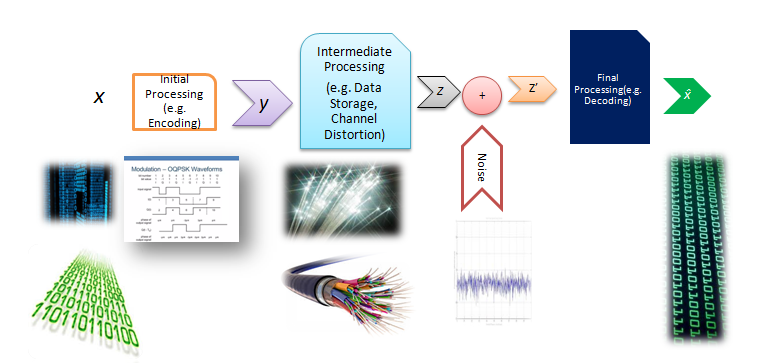
\includegraphics[width=\textwidth]{./Figures/comm_block.png}
  \caption{The general block diagram depicting the processing and recovery of data}
  \label{fig:comm_block}
\end{figure}

Ideally, we want the retrieved data $\hat{x}$ to be equal to the original data $x$ so that the error e defined as $x-\hat{x}$  is $0$; however, this is mostly unachievable due to various factors; noise, interference, hardware nonlinearities such as amplifier saturation. In addition to these external factors that are normally not in our control, there are also limitations inherent in the assumptions and models we employ that may not be adequate in capturing the complexities of the system. Hence, we try to minimize the error through various algorithms and signal processing techniques that have solid mathematical foundations. Nonetheless, these traditional techniques are as good (or bad) in capturing the complexities of our data as our models and assumptions! \\
The use of deep learning can greatly enhance error optimization. The Neural Network learns the model on its own by fitting the training data –labeled or unlabeled- into the model to minimize a particular loss function; this eliminates the inefficiencies that were concomitant with the modeling the system. By iterating through the batches of training data for a sufficient number of epochs, the neural network finds the optimal sets of weights that result in minimal loss. We can view the neural network as the model in itself! But, care must be taken in generalizing this statement; the caveat here is that nonlinear models can only be learned using neural networks with nonlinear activation functions!\\
In communication systems, when the (modulated) data is transmitted through a channel (Copper Wires, Optical Fibers, Air, Water e.t.c ), it is convolved with the channel’s impulse response and corrupted by noise and disturbances. Data at the receiver is vastly different than the one that was originally transmitted. Hence, the receiver is encumbered with the additional task of deconvolving and the denoising the received data. If it were not for the noise and channel impulse response, the received data could have been demodulated to $100\%$ accuracy ($0$ BER) by merely reversing the explicit processes that take place at the modulator and the transmitter. The block diagram for an OFDM system Figure \ref{fig:trad_ofdm} is given below: \\
\begin{figure}[htbp]
  \centering
  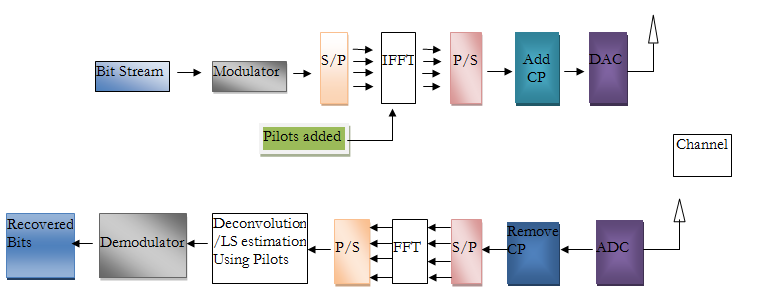
\includegraphics[width=\textwidth]{./Figures/trad_ofdm.png}
  \caption{A traditional single-user OFDM system}
  \label{fig:trad_ofdm}
\end{figure}
The effects of noise and channel distortion are highly nonlinear. This is why the use of linear operations to deconvolve and de-noise the received signal only yields limited success. The ability of the neural network to learn the nonlinear features of a system can be used to great advantage. Nonlinear activation functions like ReLU, Sigmoid, Tanh enable the network to learn complex features that would otherwise be overlooked by traditional methods. In the case of OFDM, we can transmit known data bits through the channel, save the corresponding received signals, and train the neural network using this determinate data.
\begin{figure}[htbp]
  \centering
  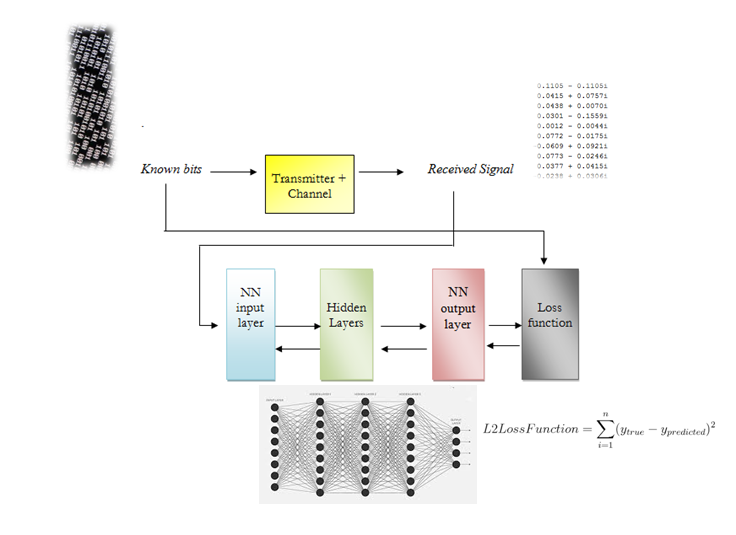
\includegraphics[width=\textwidth]{./Figures/comm_dnn.png}
  \caption{The Receiver is replaced by a Dense Neural Network (DNN)}
  \label{fig:comm_dnn}
\end{figure}
To minimize the loss function, the neural networks updates its weights using optimizers such as Stochastic Gradient Descent (SGD) and Adam’s optimizer, and in the process, learns these two things about the system:
\begin{enumerate}
\item The processes that take place on the transmitter side (e.g., Modulation, CP addition, Pilots, etc.).
\item The features of the channel and the noise that distort the transmitted data
\end{enumerate}
Once the loss has been minimized to a sufficient degree, we use the trained neural network to replace the entire receiver side except DAC. This is illustrated in Figure \ref{fig:comm_dnn} and Figure \ref{fig:comm_comparison}.\\
We also extend the block diagram above for multi-user detection, in which a single receiver recovers the data bits transmitted from 2 independent users using the Non-Orthogonal Multiple Access (NOMA) scheme. 
\begin{figure}[htbp]
  \centering
  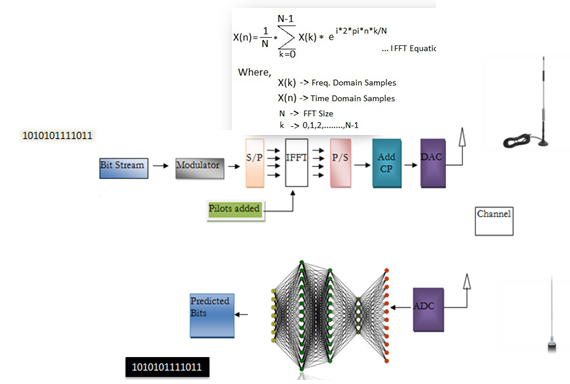
\includegraphics[width=\textwidth]{./Figures/comm_comparison.png}
  \caption{A complete OFDM system with a DNN as its receiver}
  \label{fig:comm_comparison}
\end{figure}
\subsection{Application in Bioinformatics}
For medical applications, we are working towards early diagnosis of Parkinson’s disease (PD). It affects more than 6 million people worldwide and is the second most common neurodegenerative disease after Alzheimer’s disease. There are a myriad number of symptoms for Parkinson's and these symptoms of PD progressively worsen over time, leading to a stark loss in quality of life, and a significant reduction in life expectancy. A detailed account of the Parkinson's symptoms is shown in Figure \ref{fig:park_symp}.
\begin{figure}[htbp]
  \centering
  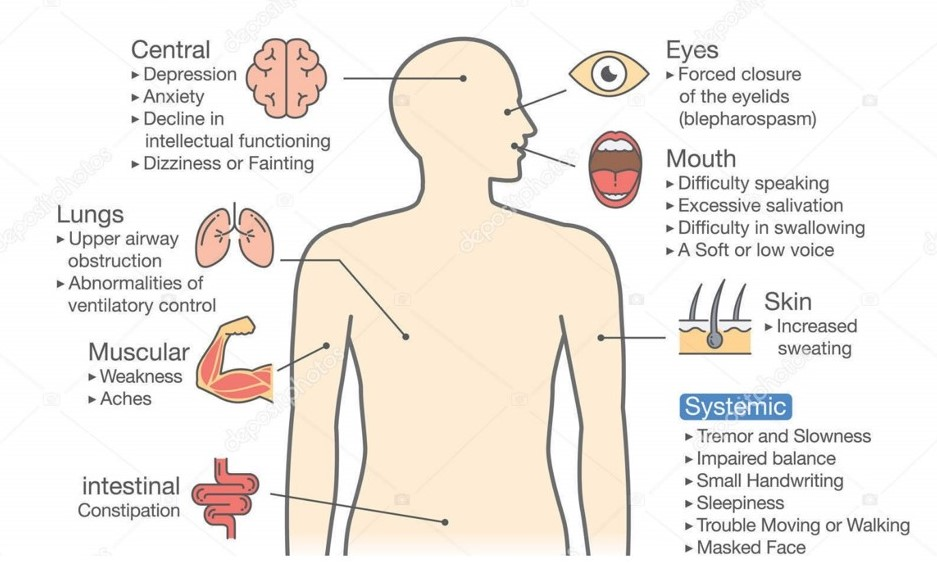
\includegraphics[width=\textwidth]{./Figures/park_symp.jpg}
  \caption{An Illustration of Parkinson's Symptoms}
  \label{fig:park_symp}
\end{figure}
Receiving a timely and accurate diagnosis is paramount for patients because access to treatments could improve their quality of life \cite{global2002factors}. So far, the traditional methods of diagnosing PD are based on subjective clinical assessments of patient’s symptoms. However, research has shown that around 25\% of this diagnosis are incorrect when compared to the results of post-mortem autopsy \cite{pahwa2010early}. These diagnoses are difficult because there are other diseases that may appear similar to PD and symptom severity may fluctuate over time \cite{pahwa2010early}. Adding to that, patients In this project, we explore the possibility of using smartPhone data collected by SageBionetworks, and made public under the umbrella of mPower study, to diagnose people with PD \cite{bot2016mpower}. Such an approach frees the diagnosis process from sporadic clinical trials and gives one the ability to do it anytime one wants. Also, this lets us explore the possibility of using deep-learning models for diagnosis task, which may improve significantly on the previous results.
\begin{figure}[htbp]
  \centering
  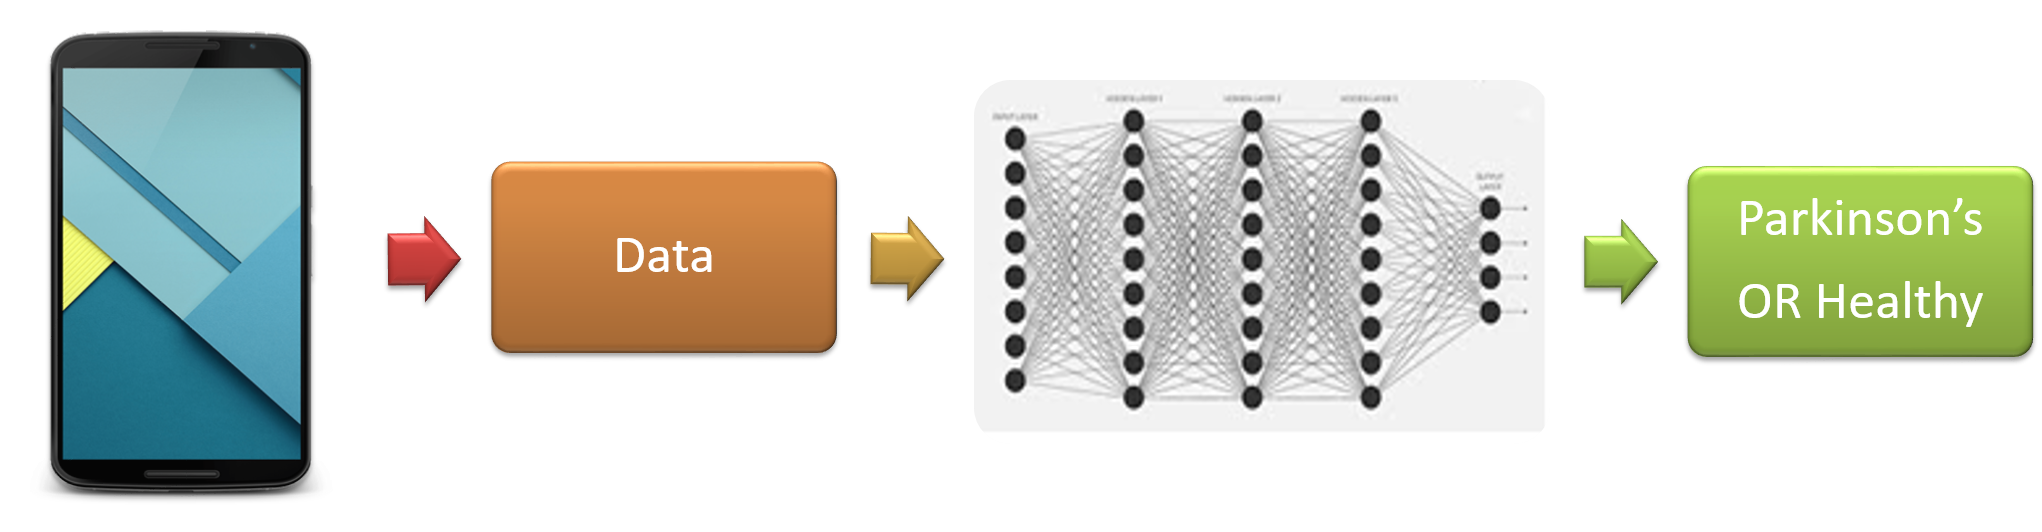
\includegraphics[width=\textwidth]{./Figures/park_dnn.png}
  \caption{A General Block Diagram for the Parkinson's Diagnosis}
  \label{fig:park_dnn}
\end{figure}

The model that we propose for the detection for the early diagnosis of Parkinson's is to optimize a Deep Learning Model that takes in data from Smartphone (Here we use the data already collected under the mPower study) and makes predictions based on this data input as shown in Figure \ref{fig:park_dnn}.
\section{Social Benefits And Relevance}
Information processing systems and health are at the heart of today’s globalized world. Our project targets two very important areas of social significance. If we are able to achieve better performance in these applications, we will impact a great number of people who use these technologies in their everyday lives.

Specifically, the application in Bioinformatics has great potential to affect people's quality of life. The traditional method for Parkinson's diagnosis is clinical diagnosis which is cumbersome and even then misclassifies 25\% of Parkinson's cases \cite{pahwa2010early}. Also, given that Parkinson's shares many of the symptoms with other diseases, patients usually are not motivated to go for a full-fledged clinical diagnosis process, which may lead to worsening of Parkinson's until the point of no recovery. However, if we are able to achieve a good enough performance on our project, we may be able to provide a rough heuristic (if not a complete diagnosis) for people to get themselves professionally checked for PD and that kind of early diagnosis can dramatically improve people's quality of life \cite{pahwa2010early}. 
\section{Goals}
Since this was primarily a research project, our goals were intended to evolve with time as we were to complete our initial deliverables and sift through a sufficient amount of research papers and other resource materials. For communication systems, our primary goal was to first minimize the Bit Error Rate (BER) for complex channel models in simulation for different communication systems (e.g., OFDM, NOMA), and compare them with the traditional methods of equalization; this was somewhat achieved. 

With regards to application in bioinformatics, we targeted the early and easy access self-monitoring of PD using smartphones. We aimed to build towards developing deep learning models which could be deployed on smartphones and can efficiently predict if people have PD using smartphones. Specific activities designed to trigger Parkinson's symptoms were to be performed and recorded on smartphones, which were then to be input to our Deep Learning model giving us the predictions.
\section{Objectives}
Our objective was to achieve the performance of the Neural Network that would be on par with the traditional methods. Once that was attained, we added complexities to our system so that the implementation of the network would become more accurate and more practical.  
\section{Outcomes}
The areas we are working on have a big part to play in the modern world. If we are able to improve on the performance of these algorithms, it will have direct implications on the Information Processing tasks and the Health of people all around the world. This could potentially mean a better world for all of us.
\section{Deliverables (Outputs)}
\textit{As our main motive is to improve on the hand-crafted algorithms in Information Processing and health, for both of our investigations: one into modulation and demodulation blocks of communication systems and the other into diagnosis of PD using smart phone data, we intend to deliver functional and trained deep neural networks which are able to perform the tasks mentioned. We also intend to compare the performance of our frameworks with current hand-crafted algorithms.}
\section{Timelines and the distribution of work}
\begin{figure}[htbp]
  \centering
  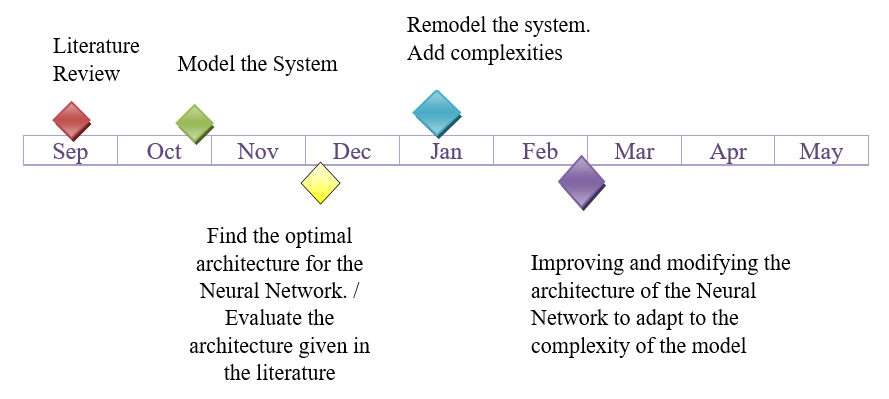
\includegraphics[width=\textwidth]{./Figures/timeline.png}
  \caption{The general summary of the timeline of our work}
  \label{fig:timeline}
\end{figure}
For application in communication systems, we had modeled the OFDM system by the end of September. It took us merely a week to verify the results of the paper our work depended on which consisted of training a Dense Neural Network with the specified architecture. The only deviation from the paper was that we did not use WINNER II and instead used Real Gaussian Channel unchanging across frames. In November, we made the channel complex and increased the number of channel variations, and recorded results for different SNRs. Until December, we worked on Single User Detection. However, in January, we decided to extend our work to the multi-user system and used NOMA. By February, we had tried different architecture for the increased complexity of the system. We found out that the architecture that gave us the best results was a mere extension of the DNN we used for single user detection. We added more neurons to our networks and added a dropout layer to prevent overfitting. In March and April, we compared the performance of our Neural Network against the benchmarks set by the traditional methods. 

For application in bioinformatics, we had reviewed the literature and gained access to the mPower study data. By the End of October, we were successful in restructuring the data to input it into our model. By December, we had successfully implemented the spline CNN \cite{balestriero2018spline} for the classification of Parkinsons's voice data recordings. Later, in January, we implemented a policy for the reclassification of data according to a fixed number of recordings per person. After this policy implementation, we moved on to the implementation of an Evidence Aggregation Model to finally output the predictions for each person. In March and April, we compared the performance of our Neural Network architecture against the benchmarks set by the traditional methods.
 % Introduction 

% Chapter 2

\chapter{Background} % Write in your own chapter title
\label{Chapter2}
\lhead{} % Write in your own chapter title to set the page header

\section{Literature Review}
\subsection{Application in Communication Systems}
During recent years, researchers have experimented with various neural network architectures to achieve optimal results. The simplest of architectures that have been used is a DNN with dense, fully connected layers. Generally, the number of hidden layers is kept to a minimum (3-4) as back propagation attenuates with the increasing number of layers. In communication systems, the problem is treated as a regression one instead of a classification one; hence the loss function used to train the neural networks for relevant applications is L2 norm instead of Softmax or Cross Entropy. Recent publications corroborate that for WINNER II channel model with AWGN noise in OFDM systems, the neural networks work slightly better than LS estimation or MMSE for 64 symbol pilot, and significantly better with an 8 symbol pilot without the use of a Cyclic Prefix (CP) \cite{ye2018power}.

Nonetheless, it is important to accentuate that the DNN in these works are mostly trained offline, and the bit error rates are calculated in the simulation rather than real time. More research on the use of end to end autoencoder architecture for OFDM systems has highlighted ability of the neural network to produce results comparable to MMSE and LS without the use of explicit equalizer on a single tap channel \cite{felix2018ofdm}. Moreover, the use of explicit equalizer has been observed to further improve the performance of the autoencoder \cite{felix2018ofdm}. There is also no noticeable degradation in the performance of the autoencoder if the pilot is omitted. The autoencoder architecture is also found to be robust to Carrier Frequency Offset (CFO) \cite{felix2018ofdm}. However, the discontinuity posed by the channel block to the backpropagation poses a challenge to any practical implementation of the end to end autoencoders.  

In \cite{ye2018power} and \cite{felix2018ofdm}, it is assumed that we have prior information about the channel. Specific models are used for training the neural network offline and then using it in real time. However, given the complexities of the channel, there are little prospects for improvements neural networks can bring to real-time workings of communication systems. Nonetheless, recent research into Generative Adversarial Net (GAN) is very encouraging; GAN enables the use of end to end auto encoders without any prior information about the channel \cite{ye2018channel}. 
\subsection{Application in Bioinformatics}
Parkinson’s disease is a neurodegenerative disease that can affect a person’s movement, speech, dexterity, and cognition. Physicians primarily diagnose Parkinson’s disease by performing a clinical assessment of symptoms. However, misdiagnoses are common. Research has shown that around 25\% of these diagnoses are incorrect when compared to the results of post-mortem autopsy \cite{pahwa2010early}. One factor that contributes to misdiagnoses is that the symptoms of Parkinson’s disease may not be prominent at the time the clinical assessment is performed \cite{schwab2018phonemd}. Another problem is the cumbersome process that discourages people from getting a clinical Parkinson's diagnosis, which may lead to worsening of Parkinson's until the point of no recovery. However, if we are able to achieve a good enough performance on our project, we may be able to provide a rough heuristic (if not a complete diagnosis) for people to get themselves professionally checked for PD and that kind of early diagnosis can dramatically improve people's quality of life \cite{pahwa2010early}. 

We are working on a deep learning approach to distinguish healthy patients from Parkinson’s patients using open-source data from mPower study \cite{bot2016mpower}. Machine Learning algorithms have already been applied to diagnose other diseases as well for example, Breast Cancer \cite{zheng2014breast}, cardiac risk factors \cite{oresko2010wearable}, skin cancer \cite{esteva2017dermatologist} and depression \cite{suhara2017deepmood}.

The data we are using consists of four different activities which are walking, tapping, memory and voice \cite{bot2016mpower}. Previous work on this data has achieved very impressive performance, i.e., 0.85 area under characteristic curve (AUC) \cite{schwab2018phonemd} using all modes of data and only 0.56 AUC using only voice data. This previous work uses expert hand-crafted features \cite{arora2015detecting} which may be limiting the full potential of this data as these features can be suboptimal. Our goal is to implement an end-to-end deep learning algorithm to explore the options for better discrimination between healthy and Parkinson’s patients. % What to Write 

% Chapter 3

\chapter{Methodology and Tools} % Write in your own chapter title
\label{Chapter3}
\lhead{} % Write in your own chapter title to set the page header

\section{System Level Design}
\subsection{Application in Communication Systems}
Traditional methods for data recovery include channel estimation through the use of pilots. In that, LS estimation or MMSE is used. At first, we investigate the performance of Deep Learning architecture for a constant, single tap channel with white noise at specified SNR.   \\
Then, we increase the number of channel taps to 8 and make a Gaussian channel. By varying channel parameters and types (No of Channel Realizations, Fading or Non fading etc.), we repeat the analysis. \\
We then use DNN to recover data bits transmitted from two different users with non-orthogonal resource allocation, at a single receiver
\begin{figure}[htbp]
  \centering
  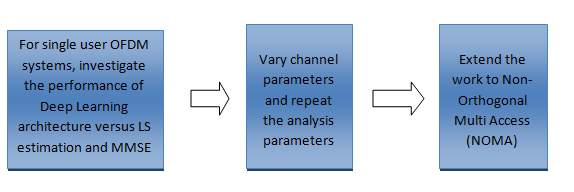
\includegraphics[width=\textwidth]{./Figures/comm_design.png}
  \caption{System level design for Communication Systems}
  \label{fig:comm_design}
\end{figure}
\subsection{Application in Bioinformatics}
Traditional methods for Parkinson's diagnosis involve a subjective clinical diagnosis. However, through the use of mPower data \cite{bot2016mpower}, we intend to augment that process with an easy-to-use predictive Neural Network architecture. We do that by understanding the data provided to us first and then apply Machine Learning techniques with hand-crafted people to generate initial results.\\
Then we replace those networks with more sophisticated Deep Learning Models and improve upon those results.\\
After that, we move towards End-to-End Deep Learning which removes all the steps required to prepare features for input to our model.
\begin{figure}[htbp]
  \centering
  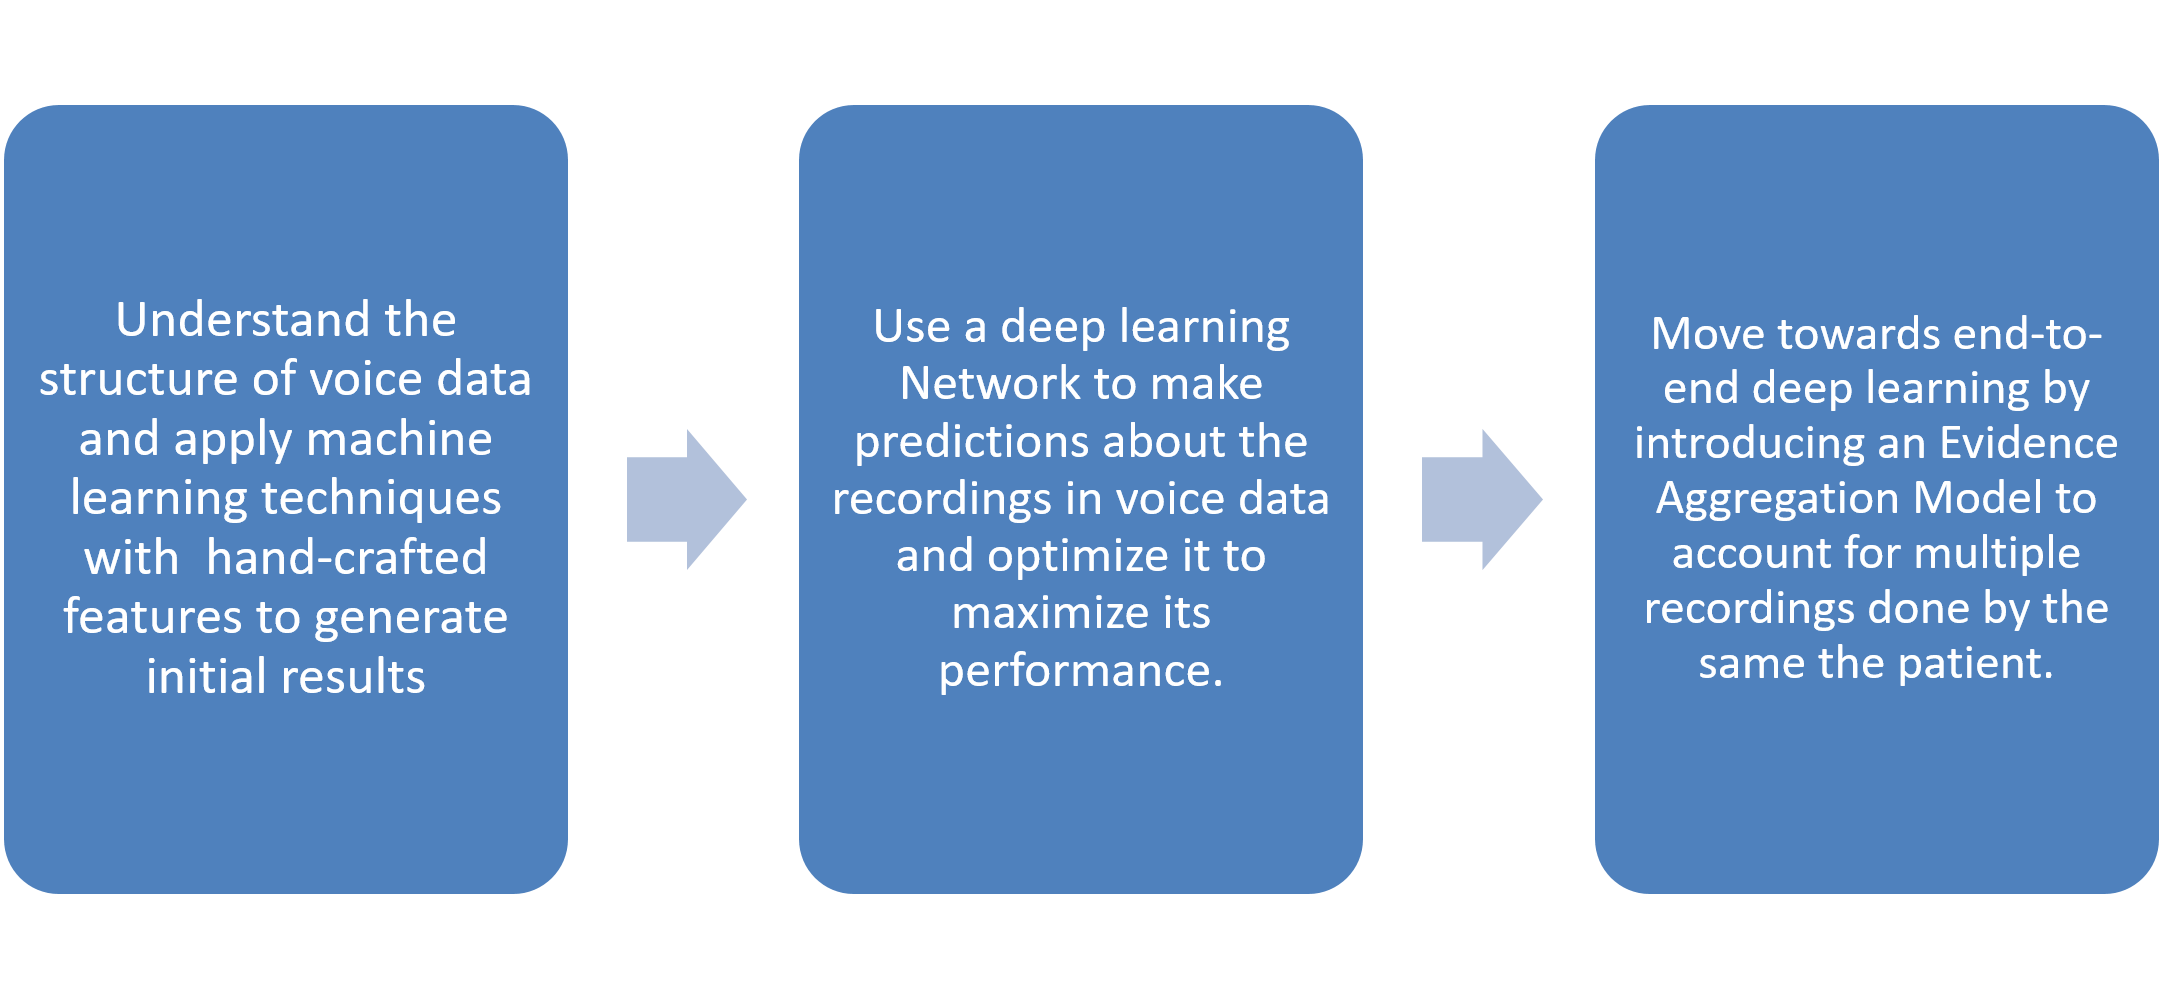
\includegraphics[width=\textwidth]{./Figures/park_method.png}
  \caption{System level design for Bioinformatics}
  \label{fig:park_method}
\end{figure}
\section{ Tools/Instruments}
\subsection{Simulation Software Packages}
We used the following sofwares/libraries for our applications:
\begin{itemize}
\item MATLAB
\item Python
\item Tensorflow
\item Keras
\item Scipy 
\item Numpy
\item Scikit-Learn
\end{itemize}
\subsection{Hardware Instruments}
We used \textbf{SOHRAB} Cluster at LUMS for our our simulation process. Its specifications are:\\
4 way SMP 48 Core E7-4830 v3 @ 2.10GHz, 256 GB RAM (Raid 10) 5*1.2 Tb - 3.3 Tb storage, Grid K40M GPU
 % Experimental Setup

% Chapter 4

\chapter{Project Implementation and Simulation} % Write in your own chapter title
\label{Chapter3}
\lhead{} % Write in your own chapter title to set the page header

\section{Simulation Setup}
\subsection{Application in Communication Systems}
\subsubsection{OFDM Systems}
Firstly, the data is generated in Matlab for traditional OFDM frames. There are 64 subcarriers. The data and pilot bits, both of size 128, are generated independently and are then mapped onto QPSK modulation scheme resulting in sequences of size 64 symbol. After converting them to time-domain by taking their 64-point IFFT,  the cyclic prefix of size 16 symbols is added to both sequences after which they are concatenated. The frame of size 180 symbols is convolved with the channel impulse response, and then the Additive White Gaussian Noise is added to it. The cyclic prefix is then removed, and the pilot and data sequences are extracted. The resulting frame size of 128 symbols is ready for analysis.\\
We investigate three techniques used to recover the original data:
\begin{enumerate}
\item \textbf{Least Squares (LS) Estimation:} In this approach, the pilots are explicitly used for Channel State Information (CSI) estimation. The DFT of the channel is obtained by dividing the 64-point FFT of the pilot in the received frame by the 64 point FFT of the transmitted frame. The estimated modulated data is then obtained by dividing the 64-point FFT of the data portion from the received frame and the estimated DFT of the channel impulse response. The estimated modulated data can then be mapped back to 128 bits using QPSK constellation diagram.
\item \textbf{Time Domain Processing:} This is similar to the above-mentioned scheme except for the method of estimating H. Using our assumption on the number of channel taps, the convolution can be used to derive a matrix equation linking the channel impulse response, transmitted pilot sequence, and the received pilot sequence. Once h[n], its DFT can be computed, and the remainder of the process is the same as before.
\item \textbf{Deep Learning:} Here, we use a neural network whose architecture is explained in the diagrams below. The neural network is trained using Keras libraries for Tensorflow in python.  The details of the Neural Network Architecture are illustrated in Figure \ref{fig:comm_16_bit} and Figure \ref{fig:comm_128_bit}.
\end{enumerate}
\begin{figure}[htbp]
  \centering
  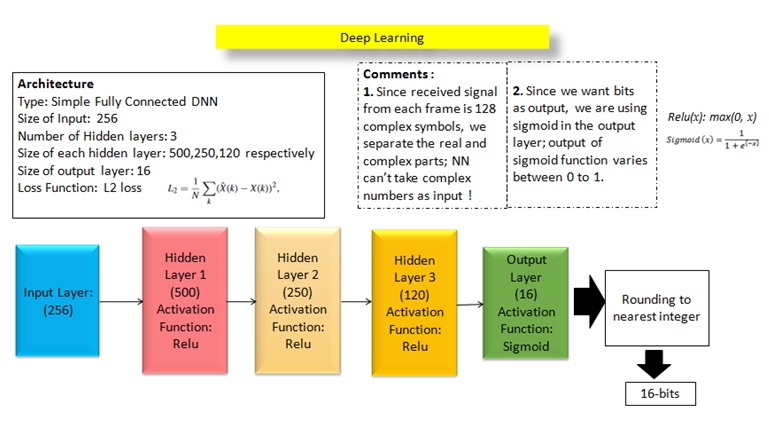
\includegraphics[width=\textwidth]{./Figures/comm_16_bit.png}
  \caption{A single Neural Network block to recover 16 bits}
  \label{fig:comm_16_bit}
\end{figure}
\begin{figure}[htbp]
  \centering
  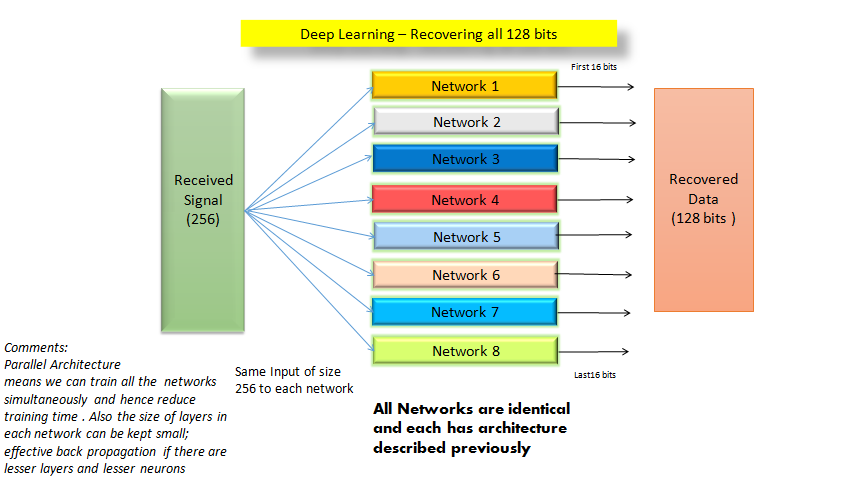
\includegraphics[width=\textwidth]{./Figures/comm_128_bit.png}
  \caption{The whole architecture that recovers all 128 bits}
  \label{fig:comm_128_bit}
\end{figure}
\subsubsection{NOMA Systems}
Using the structure for simulation for OFDM system as a skeleton, we extend our work to Non-Orthogonal Multiple Access (NOMA) system. We keep our work restricted to 2 users only. However, since the interference from two users increases the complexity of the problem at hand, we start with 16 subcarriers and a 3 tap channel to observe the trends, and then simulate for 64 subcarriers and 8 tap channel systems to confirm those trends.\\
The frame structure for NOMA is sufficiently similar to the one for OFDM system. For 16 subcarrier system, 32-bit data is converted to 16 complex symbols using QPSK modulation. Then 16 point IFFT is carried out on these symbols. Moreover, as in the case of OFDM, the pilot bits, equal in length to the data bits (true for most of our work) is QPSK modulated and converted to time-domain. The pilot is then concatenated with time domain data. However, this time space is reserved for the pilot of the other user. This ensures that while the data of the two users are non-orthogonal, the pilots are orthogonal in time. This is illustrated in figure \ref{fig:comm_noma}.\\
\begin{figure}[htbp]
  \centering
  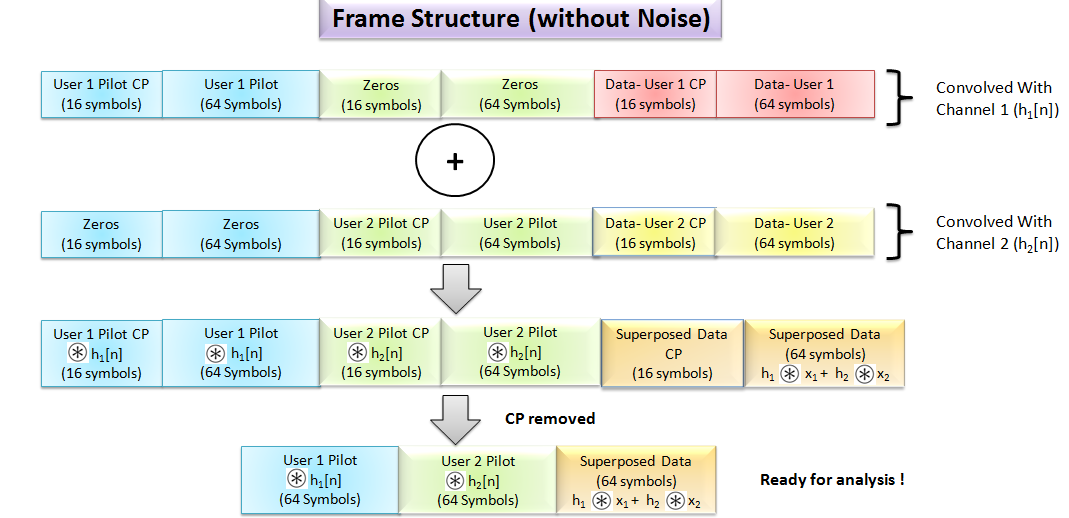
\includegraphics[width=\textwidth]{./Figures/comm_noma.png}
  \caption{Frame Structure for NOMA system: the pilot symbols are preserved despite interference}
  \label{fig:comm_noma}
\end{figure}
After interference, Gaussian noise is added to signal before it is passed onto the receiver. Unless otherwise specified, the simulations must be assumed to have been carried out at $20$ SNR. \\
The method for theoretical estimation of BER is somewhat different than the one used for OFDM systems. As before, we estimate the DFT of the channel impulse response using the pilots. We then use Maximum Likelihood estimation at a subcarrier level in frequency domain to infer which of the four possible symbols was transmitted. This can be illustrated in the following equations:\\
$$Y_{(data)}=H_1X_{1(data)}+H_2X_{2(data)}+Z$$
where,\\
$$X_1,X_2\in[e^{j(2k+1)\frac{\pi}{4}}] \mid k\in\{-2,-1,0,1\}$$
$$F^{-1}(Z)\in \mathcal{N}(0,\sigma^2)$$
The Conditional Distribution on $Y$ is given by:\\
$$f(Y\mid X_1,X_2,H_1,H_2,\sigma^2)\propto e^{-\frac{|Y-H_1X_1-H_2X_2|^2}{2\sigma^2}}$$
$$\implies \hat{X}_1 = \arg \max_{x_1\in QPSK}f(Y\mid X_1=x_1)=\arg \max_{x_1\in QPSK}\sum_{x_2\in QPSK}f(Y\mid X_1=x_1,X_2=x_2)$$
$$\implies \hat{X}_1 = \arg \max_{x_1\in QPSK}\sum_{x_2\in QPSK}e^{-\frac{|Y-H_1x_1-H_2x_2|^2}{2\sigma^2}}$$
Similarly,\\
$$\hat{X}_2 = \arg \max_{x_2\in QPSK}\sum_{x_1\in QPSK}e^{-\frac{|Y-H_1x_1-H_2x_2|^2}{2\sigma^2}}$$

To get a tighter theoretical limit on the BER, we also used separately the actual CSI (stored in a csv file) rather than the CSI estimate obtained from the pilots. \\
As far as the Deep Learning architecture is concerned, we investigated several models including the auto-encoders. However, the architecture that gave us the best results was merely a modification of the Dense Neural Network used in the single user case. We carried out our experiments for 16- Subcarrier systems and 64-Subcarrier Systems, architecture for which is shown in figure \ref{fig:comm_nomaarch}
\begin{figure}[htbp]
  \centering
  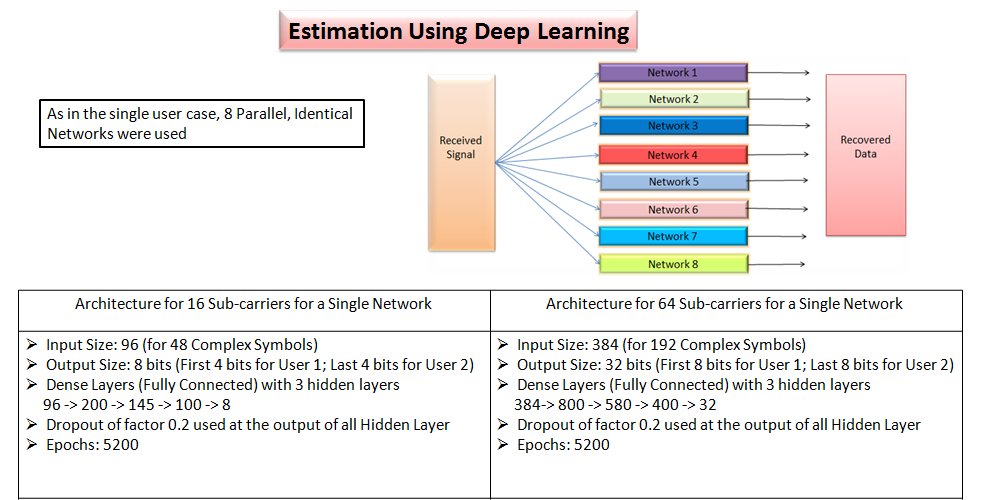
\includegraphics[width=\textwidth]{./Figures/comm_nomaarch.png}
  \caption{Deep Learning architectures used for NOMA systems}
  \label{fig:comm_nomaarch}
\end{figure}
\subsection{Application in Bioinformatics}
For this application, we first need to understand the structure of the data, and then we will move onto devising architectures for End-to-End Deep Learning. 
\subsubsection{Struture of mPower Data}
The mPower data \cite{bot2016mpower} is consists of four types of activities: Walking, Voice, Tapping and Memory. Figure \ref{fig:park_flow} illustrates the structure of mPower data. For our purposes, we limit our attention to Voice data. These four types of activities are specifically designed to trigger Parkinson's symptoms response. Each activity is recorded via the following processes:
\begin{itemize}
\item \textbf{Walking}: Subjects walk 10 steps with a phone in their pocket. Phone's Gyroscopic measurements are recorded during the whole activity. This activity is intended to capture irregularities in walking if any.
\item \textbf{Voice}: Subjects record 10 seconds of voice into the microphone of their cell-phone. This data is intended to capture the jitter or shimmer in the voice if any.
\item \textbf{Tapping}: Subjects tap on two points on the phone repeatedly. The tapping positions and intervals are recorded. This data is intended to record tremor in hand motions if any.
\item \textbf{Memory}: Subjects play a guessing game. In this game, the results of pattern matching are recorded. This activity is intended to capture if the memory is in good shape since one of the symptoms of Parkinson's is loss of memory.
\end{itemize}
\begin{figure}[htbp]
  \centering
  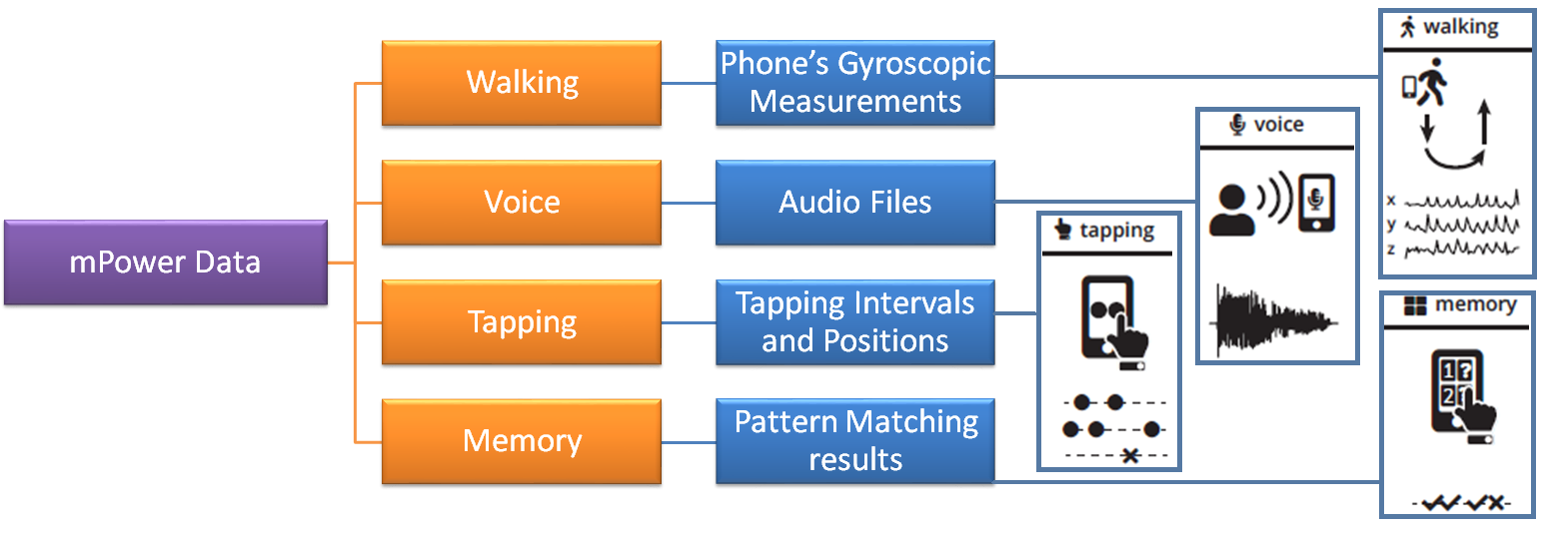
\includegraphics[width=\textwidth]{./Figures/mpower_data.png}
  \caption{The Structure of mPower Data}
  \label{fig:park_flow}
\end{figure}

\subsubsection{Structure of Voice Data}
The voice data contains 65,022 audio files in total which are organized on the basis of the time of their recording as illustrated by Figure \ref{fig:park_time}. We ignored the recordings of Parkinson's patients done just after medication, as we believe that those recordings would not provide information about Parkinson's symptoms as Parkinson's medications, suppress these symptoms \cite{schwab2018phonemd}.
\begin{figure}[htbp]
  \centering
  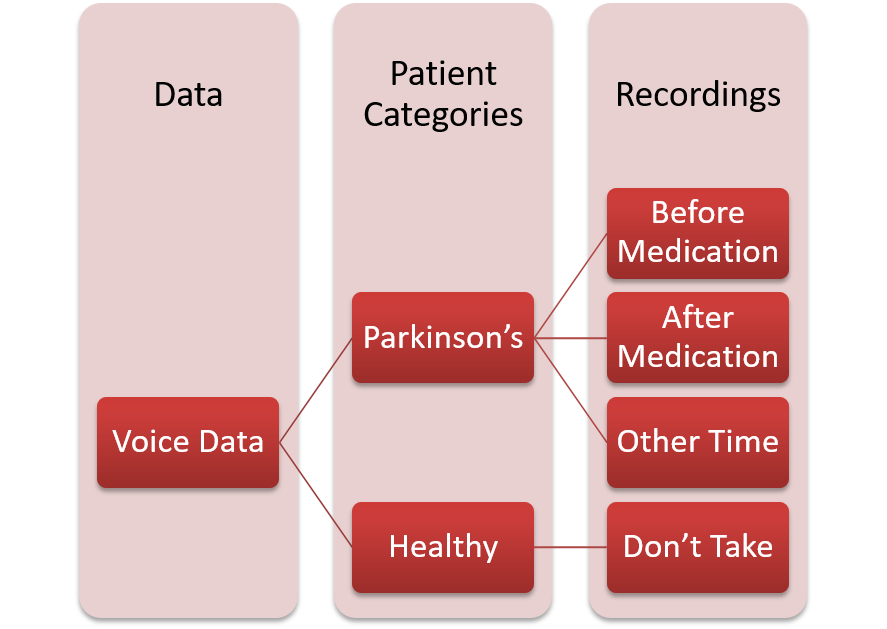
\includegraphics[width=\textwidth]{./Figures/park_time.png}
  \caption{Different types of recordings in Voice Data}
  \label{fig:park_time}
\end{figure}

However, the data available to us is imbalanced in terms of the number of people participating in the study. We observe that only 20\% of the people are clinically diagnosed by Parkinson's Disease, while an overwhelming 58\% of the recordings are attributed to that 20\ % of the people. This means that on average, people with Parkinson's have recorded more audio files as compared to Healthy people as illustrated in Figure \ref{fig:park_dist}.\\
\begin{figure}[htbp]
  \centering
  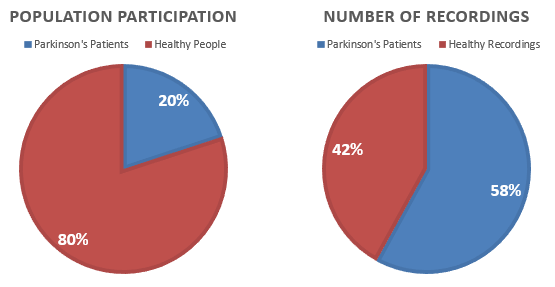
\includegraphics[width=\textwidth]{./Figures/park_dist.png}
  \caption{The Vioce Data Distribution according to PD indication}
  \label{fig:park_dist}
\end{figure}
\subsubsection{Initial Investigation with Machine Learning Models}
Initially, we assumed every recording sample independent of each other and designed a recording-level classifier. The pipeline designed for such a classifier is illustrated in Figure \ref{fig:park_pipeline}.
\begin{figure}[htbp]
  \centering
  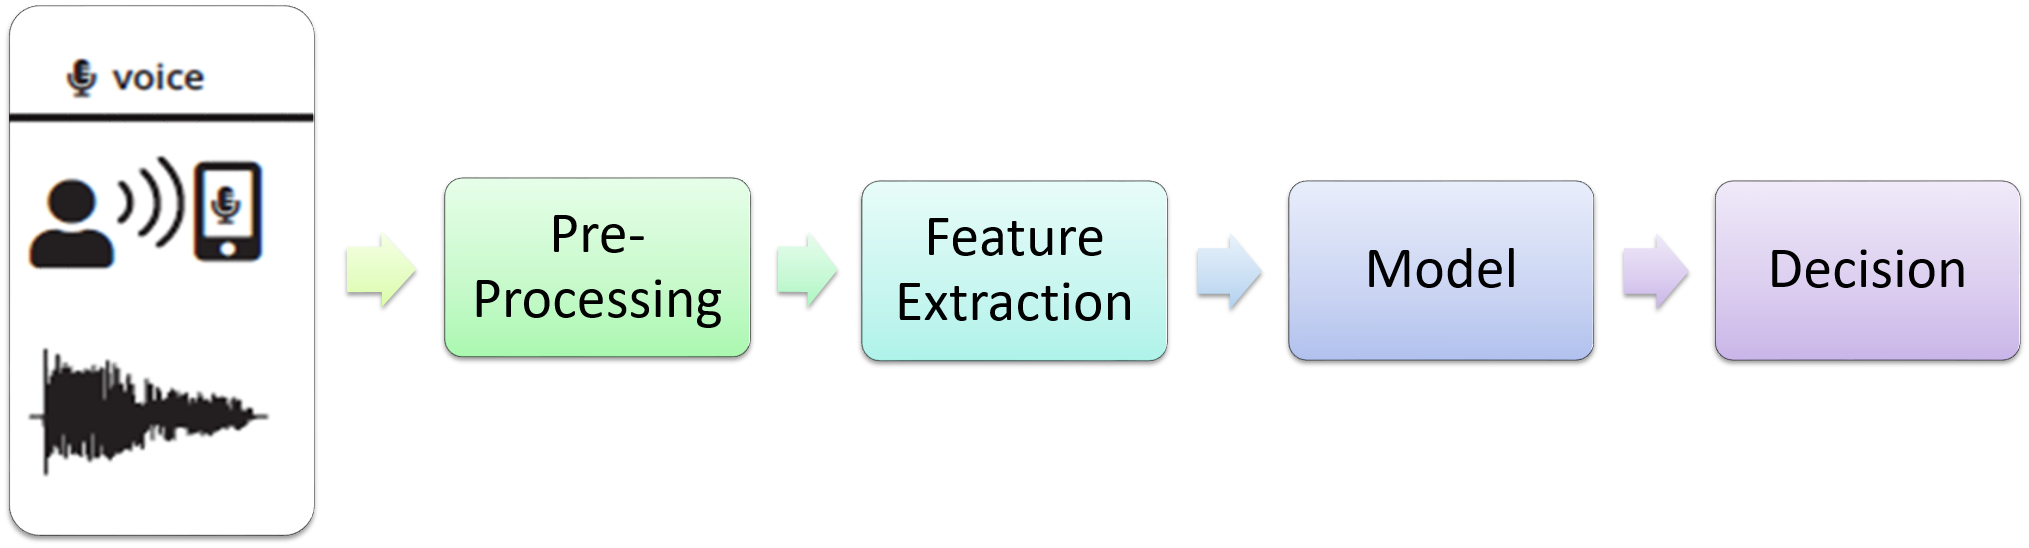
\includegraphics[width=\textwidth]{./Figures/park_pipeline.png}
  \caption{Initial Pipleline Designed for a Recording-level Classifier}
  \label{fig:park_pipeline}
\end{figure}
The following features were used for training these classifiers:
\begin{itemize}
\item Detrended fluctuation analysis \cite{arora2015detecting}
\item Mean Teager-Kaiser energy operator \cite{arora2015detecting}
\item Mel-Frequency Cepstal Co-efficients \cite{arora2015detecting}
\end{itemize}
By training these classifiers, we were able to achieve an Area Under Curve measure of 0.88 as illustrated in Figure \ref{fig:park_ini_res}, but our assumptions were wrong are there was high correlation present between two  audio-files recorded by the same patient and treating them as independent was misleading.
\begin{figure}[htbp]
  \centering
  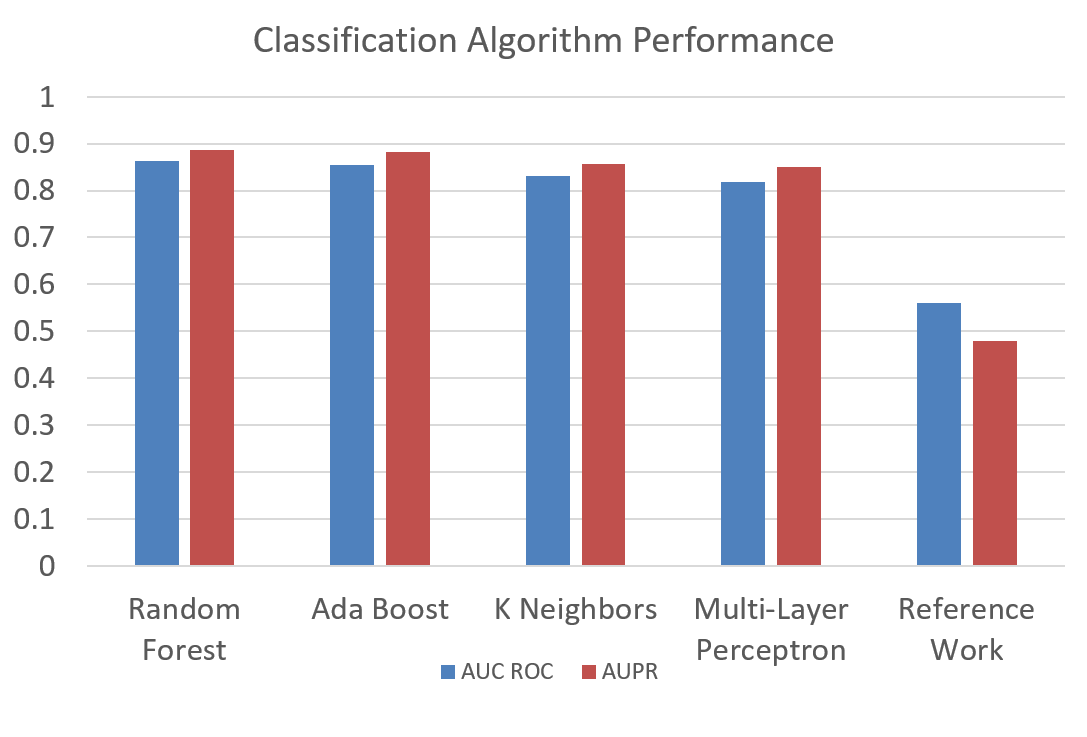
\includegraphics[width=\textwidth]{./Figures/park_ini_res.png}
  \caption{Results of Machine Learning Algorithms with Incorrect Assumption of Independence}
  \label{fig:park_ini_res}
\end{figure}
\subsubsection{Selection of a Fixed Number of Recordings per Person}
After the correction of our assumption of independence, we limited all the recordings from one particular person to either train set or the test set. Hence, a high correlation between two recordings does not affect our performance measures as all of those recordings are located entirely on one side of the split. It turns out when we limit all the recordings by one patient into either test or train dataset; the metrics drop rapidly.

The contribution of recordings by different people is very asymmetric. Some people have too many recordings, some too few. This causes a bias when training a recording level classifier as well as a person level classifier. As shown in Figure \ref{fig:park_asymm}, we see that the mode number of recordings is 3. Almost 31\% of the people have done 3 recordings, and the mean number of recordings is 11.57. 
\begin{figure}[htbp]
  \centering
  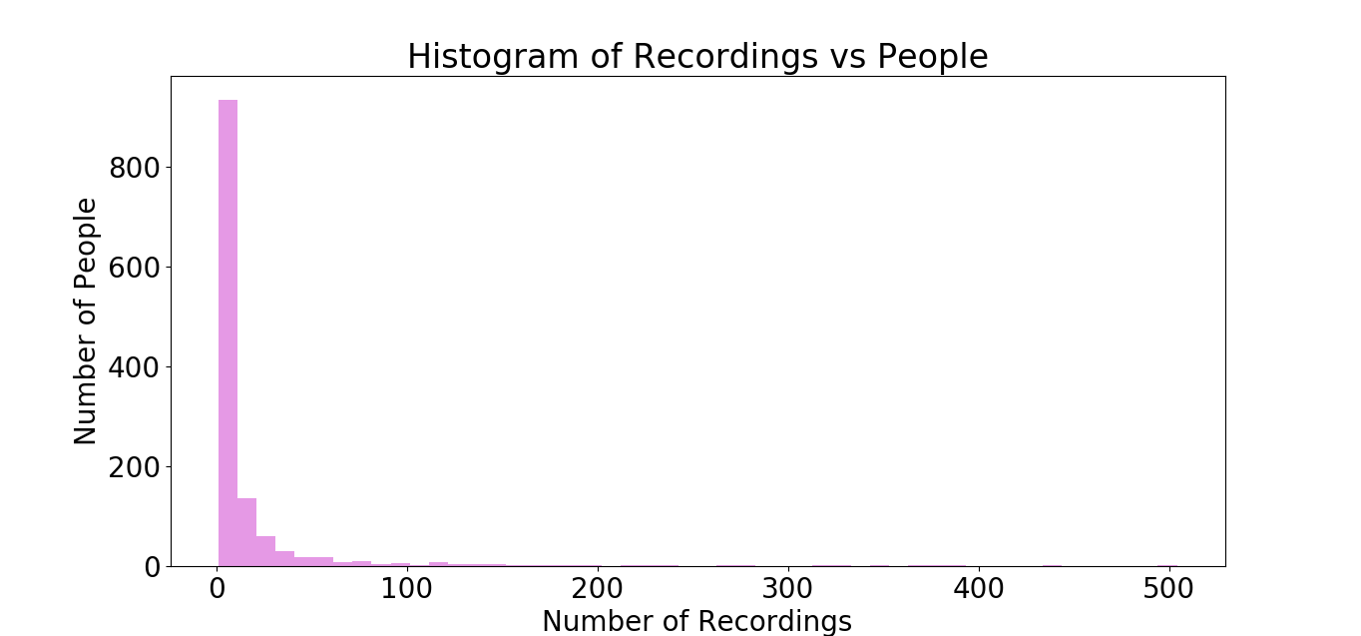
\includegraphics[width=\textwidth]{./Figures/park_asymm.png}
  \caption{Asymmetry in the Number of Recordings done by Different People}
  \label{fig:park_asymm}
\end{figure}
Therefore, we devise a policy of selecting a fixed number (let's say $k$) of recordings per person. This is done for the following reasons:
\begin{itemize}
\item People with lesser number of recordings become under-represented and provide us very less information.
\item A large number of recordings from the same person provides redundant information as the correction between two recordings by the same person is very high. This costs us in the form of un-required computation.
\end{itemize}
Therefore, we implemented this selection and tested our performance measure by selecting 2,3,4 and 5 number of recordings per person for each architecture. 
\subsubsection{Spline Convolutional Neural Network Architecture}
We use a deep neural network architecture \cite{balestriero2018spline} to classify the recordings because this architecture was designed to detect and learn features for audible data. The detailed structure for such an architecture is given in Figure \ref{fig:spline_cnn}.
\begin{figure}[htbp]
  \centering
  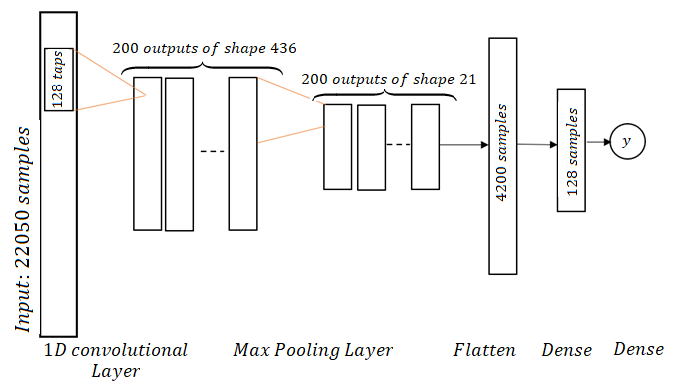
\includegraphics[width=\textwidth]{./Figures/spline_cnn.png}
  \caption{The Architecture of Spline Convolutional Neural Network}
  \label{fig:spline_cnn}
\end{figure}

The spline CNNs are a special form of regular CNNs with the change that convolutional filters are initialized as band-limited filters with several center frequencies covering the whole Frequency-space. The CNN is called spline CNN because Hermite-cubic splines are used for filter construction. The filters are constructed by first designing 1 `mother-filter' in Frequency Domain and then shifting it to cover the whole Frequency range. In our case, we use a filter of 100 Hz Bandwidth and shift it with a frequency of $\sim$10 Hz to make 200 band-limited filters. The sampling frequency we use is 2205 Hz. These 200 filters are initialized as convolutional filters in our network and then learned as we train the network. For illustration, two sample filters out of the 200 filters have been shown in Figure \ref{fig:twofils}
\begin{figure}
\centering
\parbox{6cm}{
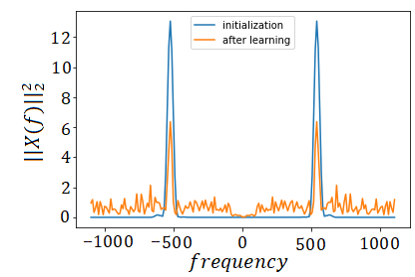
\includegraphics[width=6cm]{./Figures/park_fil1.png}
%\caption{First.}
\label{fig:2figsA}}
\qquad
\begin{minipage}{6cm}
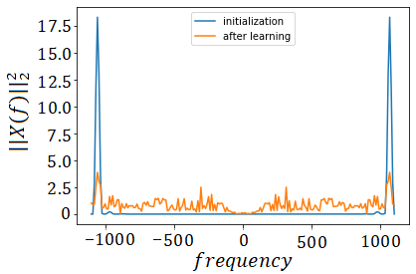
\includegraphics[width=6cm]{./Figures/park_fil2.png}
%\caption{Second.}
\label{fig:2figsB}
\end{minipage}
\caption{Sample filters for Spline-CNN}
\label{fig:twofils}
\end{figure}

\subsubsection{Evidence Aggregation Model (EAM)}
We introduced another Deep Learning Model into our pipeline to output a final prediction for each person based upon their predictions from the recording-based classifier. This updates our pipeline to the one shown in Figure \ref{fig:new_pipe}
\begin{figure}[htbp]
  \centering
  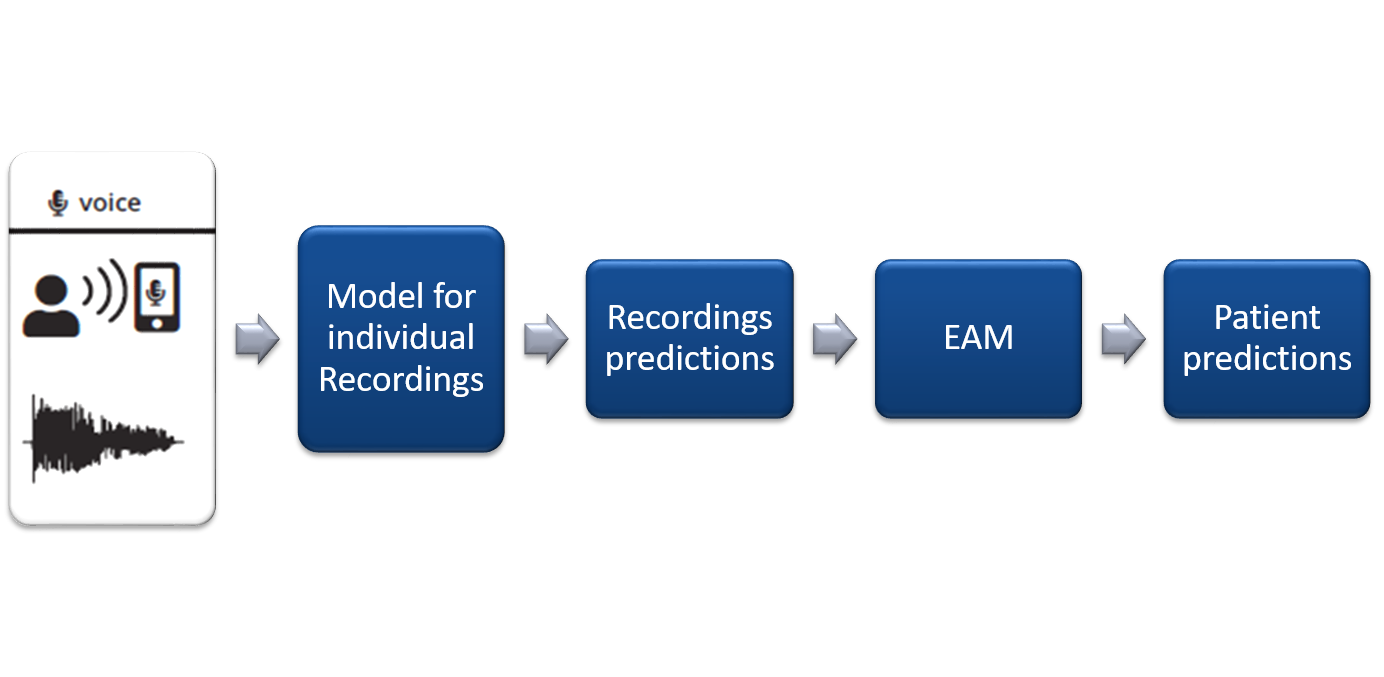
\includegraphics[width=\textwidth]{./Figures/new_pipe.png}
  \caption{New PipeLine Model after adding Evidence Aggregation Model}
  \label{fig:new_pipe}
\end{figure}
EAM is implemented as a Deep Bi-directional LSTM network, as shown in Figure \ref{fig:eam}. The work of EAM was to aggregate results from more than one models as we move towards other activities as well. However, for this setting, where we are only working with the voice data, the EAM converges to mode function.
\begin{figure}[htbp]
  \centering
  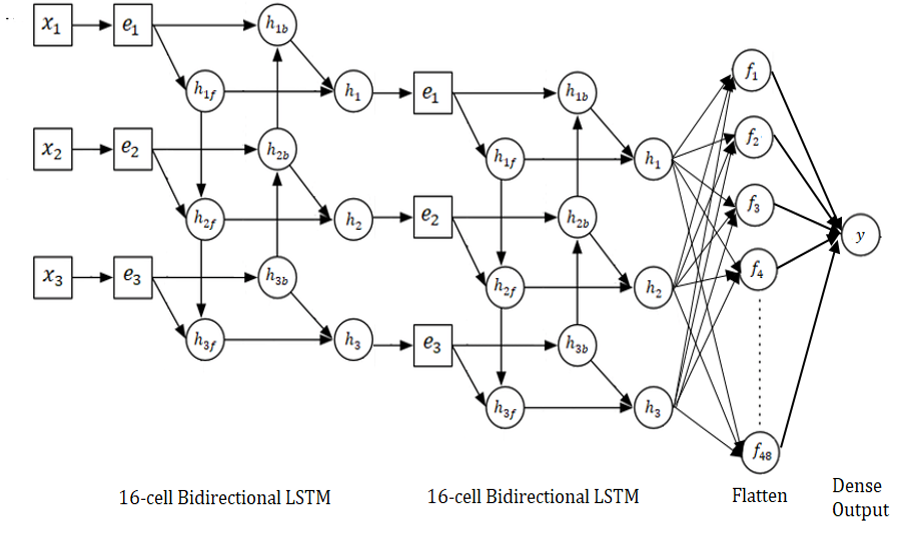
\includegraphics[width=\textwidth]{./Figures/eam.png}
  \caption{Structure of Evidence Aggregation Model}
  \label{fig:eam}
\end{figure}
\section{Simulation Results}
\subsection{Application in Communication Systems}
\subsubsection{OFDM Systems}
\begin{figure}[htbp]
  \centering
  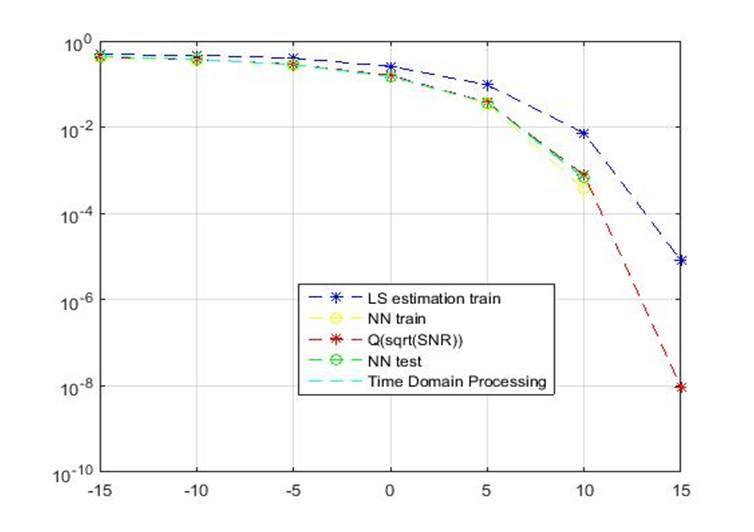
\includegraphics[width=\textwidth]{./Figures/awgn_results.png}
  \caption{Results for AWGN Channel}
  \label{fig:awgn_results}
\end{figure}
Figure \ref{fig:awgn_results} shows results for a single tap channel with Additive White Gaussian Noise (AWGN). The training data consisted of 50,000 messages while testing data consisted of 10,000 messages. The channel was unchanging across frames.  \\
We can see that Least Squares (LS) estimation fares the worst while time domain processing fares better since it utilizes the knowledge of number of channel taps used. We see that Neural Network performed the best and performed at par with Theoretical limit given by:\\
$$Q(\sqrt{10^{\frac{SNR(dB)}{10}}})$$
\begin{figure}[htbp]
  \centering
  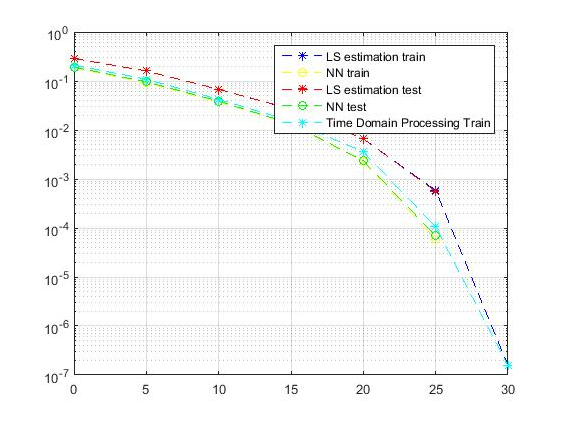
\includegraphics[width=\textwidth]{./Figures/real_8tap_res.png}
  \caption{Results for 8 tap real channel which is unchanging across frames}
  \label{fig:real_8tap_res}
\end{figure}
Figure \ref{fig:real_8tap_res} shows results for 8 tap real channel drawn from a Gaussian distribution. Again, the training data consisted of 50,000 messages while testing data consisted of 10,000 messages. The channel was unchanging across frames.  We again see that Neural Network performed the best. \\
\begin{figure}[htbp]
  \centering
  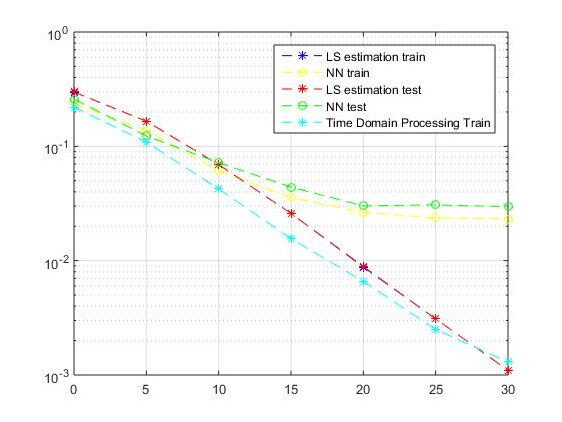
\includegraphics[width=\textwidth]{./Figures/real_8tap_chn.png}
  \caption{Results for 8-tap real channel which is changing across frames}
  \label{fig:real_8tap_chn}
\end{figure}
Figure \ref{fig:real_8tap_chn} shows results for 8-tap real channel drawn from a Gaussian distribution. As before, the training data consisted of 50,000 messages while testing data consisted of 10,000 messages. This time, the channel is changed every frame so that we have 50,000 instances of the channel. This has led to degradation in the performance of the Neural Network causing it to lag behind theoretical methods. One possible explanation could be that the neural network does not have enough examples to learn the distribution channels are drawn from.\\
\begin{figure}[htbp]
  \centering
  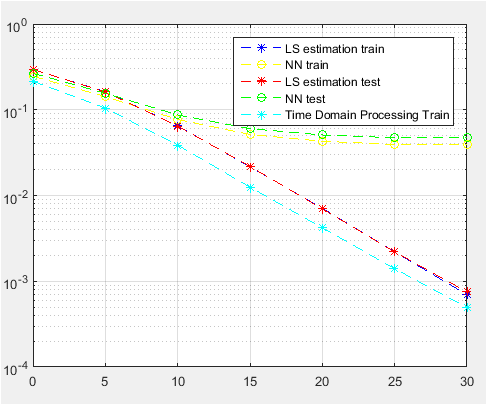
\includegraphics[width=\textwidth]{./Figures/complex_8tap_res.png}
  \caption{Results for 8 tap complex channel which is changing across frames}
  \label{fig:complex_8tap_res}
\end{figure}
Figure \ref{fig:complex_8tap_res} shows results for 8 tap complex, exponentially fading channel. Both real and imaginary parts are drawn from a Gaussian distribution and have equal energies. The training data consisted of 50,000 messages while testing data consisted of 10,000 messages. Also, the channel is changed every frame so that we have 50,000 instances of the channel. The performance of Neural Network deteriorates while the performance LS estimation and Time domain processing improves slightly.\\
\subsubsection{NOMA systems}
Since we now have to do a joint estimation of both users’ data the complexity of the problem has increased. Consequently, we had to use more neurons per layer, and we had to increase the number of epochs by a factor of 52. Therefore, we considered it prudent to carry out most of our experiments for 16 subcarrier systems and then verify them for 64 subcarrier systems.\\
\begin{table}[htbp]
  \centering
  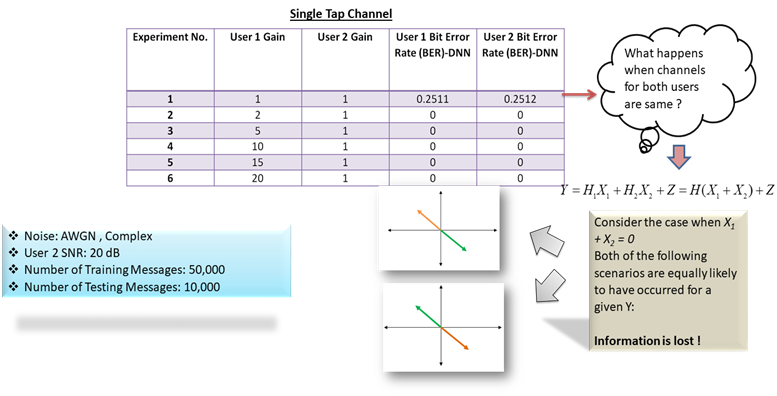
\includegraphics[width=\textwidth]{./Figures/noma_single_res.png}
  \caption{Results for Single tap Channel (NOMA)}
  \label{tbl:noma_single_res}
\end{table}
Table \ref{tbl:noma_single_res} shows results for a Single tap channel. The noise added was complex. The Signal to Noise ratio (SNR) for user 2 was maintained at 20 dB. The gain for user 1 was varied which was akin to changing its SNR. The number of training messages used was 50,000 while the number of testing messages used was 10,000. As we can see here, the neural network achieved perfect decoding of the received data. However, it was observed that when the channel for both users was same, the Neural Network failed because QPSK modulation uses sets of symbols that are $180^o$ apart in phase, that cancel out resulting in a loss of information.\\
\begin{table}[htbp]
  \centering
  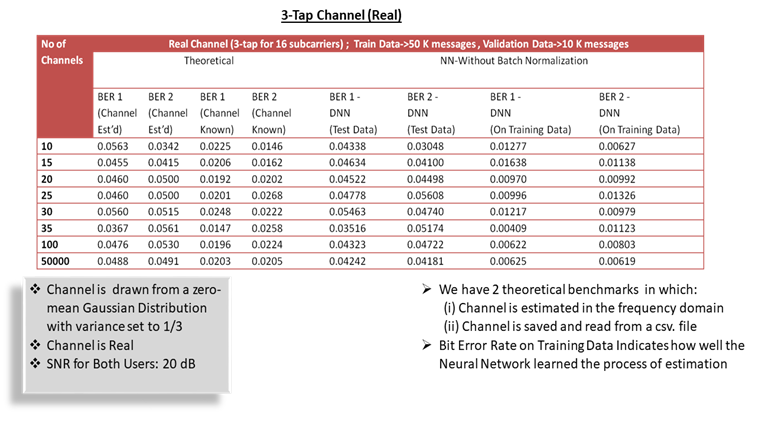
\includegraphics[width=\textwidth]{./Figures/noma_3tap_res.png}
  \caption{Results for 3-tap Real Channel (NOMA)}
  \label{tbl:noma_3tap_res}
\end{table}
\begin{figure}[htbp]
  \centering
  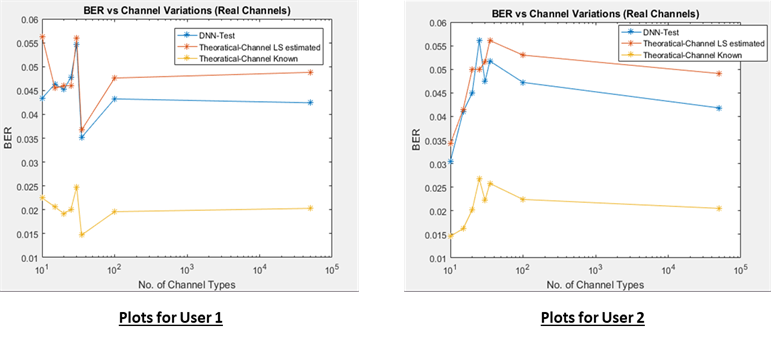
\includegraphics[width=\textwidth]{./Figures/noma_comp.png}
  \caption{Plots of BER for both users for 3-tap Real Channel against No. of Channel (NOMA)}
  \label{fig:noma_comp}
\end{figure}
Table \ref{tbl:noma_3tap_res} and Figure \ref{fig:noma_comp} demonstrate results when the number of Channel taps is increased to 3. The Channel is kept real and drawn from a zero-mean Gaussian distribution. This time, the SNR for both of the users is maintained at 20 dB. We used 2 theoretical benchmarks to gauge the performance of the Neural Network. The first method uses Least Squares Estimation in the frequency domain to estimate the channel. In the second method, the channel is saved and loaded from a .csv file and used to recover the data. Since the major hurdle in the data recovery is channel estimation, this method gives us the theoretical limit below which the bit error rate cannot possibly go. We investigated the BER against the increase in Number of Channel types or instances. The plots show that the neural network performs slightly better than the theoretical method that uses Least squares estimation of the channel. Also, we see that contrary to the case of single user detection; the neural network has also managed to learn the channel distribution as the performance of the neural network does not degrade as we increase the number of channel types. Similarly, figure \ref{fig:noma_3tap_snr} below shows that BER decreases with increasing SNR.\\
\begin{figure}[htbp]
  \centering
  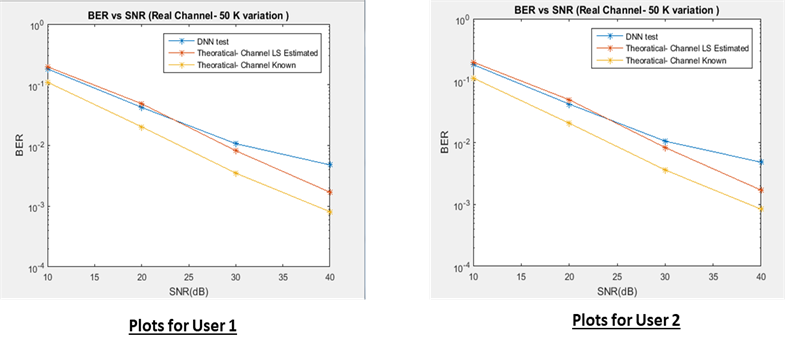
\includegraphics[width=\textwidth]{./Figures/noma_3tap_snr.png}
  \caption{Plots of BER for both users for 3-tap Real Channel against SNR (NOMA)}
  \label{fig:noma_3tap_snr}
\end{figure}
\begin{table}[htbp]
  \centering
  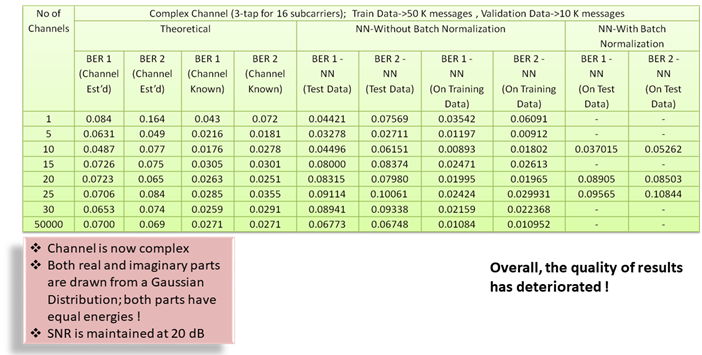
\includegraphics[width=\textwidth]{./Figures/noma_3tap_complex.png}
  \caption{Results for 3-tap Complex Channel (NOMA)}
  \label{tbl:noma_3tap_complex}
\end{table}
\begin{figure}[htbp]
  \centering
  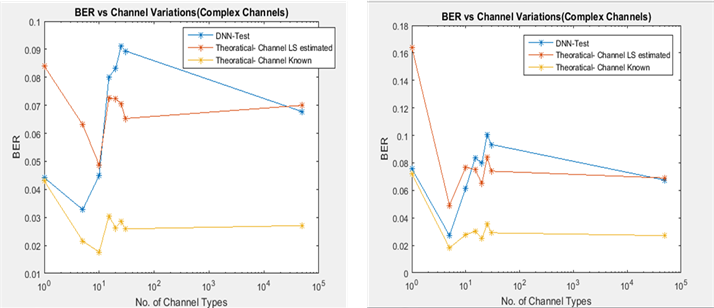
\includegraphics[width=\textwidth]{./Figures/noma_3tap_complexnochannel.png}
  \caption{Plots of BER for both users for 3-tap Complex Channel against No. of Channel (NOMA)}
  \label{fig:noma_3tap_complexnochannel}
\end{figure}
Table \ref{tbl:noma_3tap_complex} and Figure \ref{fig:noma_3tap_complexnochannel} demonstrate what happens when we make the channel complex. Both the real and imaginary parts of the channel have been drawn from a Gaussian distribution, and the energies of both parts are kept equal. We can see that the bit error rates have gone up and the overall quality of results have deteriorated. However, the Neural Network still performs at par with the theoretical method that estimates the channel using the Least Squares. \\
To confirm the robustness of our results, we extend our experiments to 64 subcarrier system, the results of which are shown in Table \ref{tbl:noma_8tap_res}. Since the Number of training, messages have been increased 10 folds, and the neurons in each layer have also been increased, the training took longer than the training in the 16-subcarrier system. Results show that the Neural Network performs slightly poorer than the theoretical methods.
\begin{table}[htbp]
  \centering
  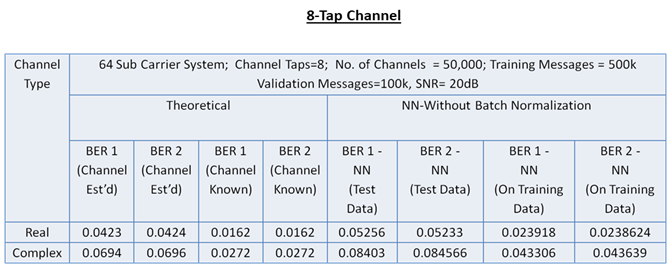
\includegraphics[width=\textwidth]{./Figures/noma_8tap_res.png}
  \caption{Results for an 8-tap complex channel varying across frames for 64 sub-carrier system}
  \label{tbl:noma_8tap_res}
\end{table}
\subsection{Application in Bioinformatics}
We compare our results to the state-of-the-art work on the same dataset by P.Schwab \cite{schwab2018phonemd} who have used Traditional Machine Learning techniques to classify between Parkinson's patients and Healthy persons.
\subsubsection{Results using Random Forest}
After the correction of our independence assumption, we were able to improve upon the reported result by using more robust hand-crafted features as shown in Figure \ref{fig:first_res}.
\begin{figure}[htbp]
  \centering
  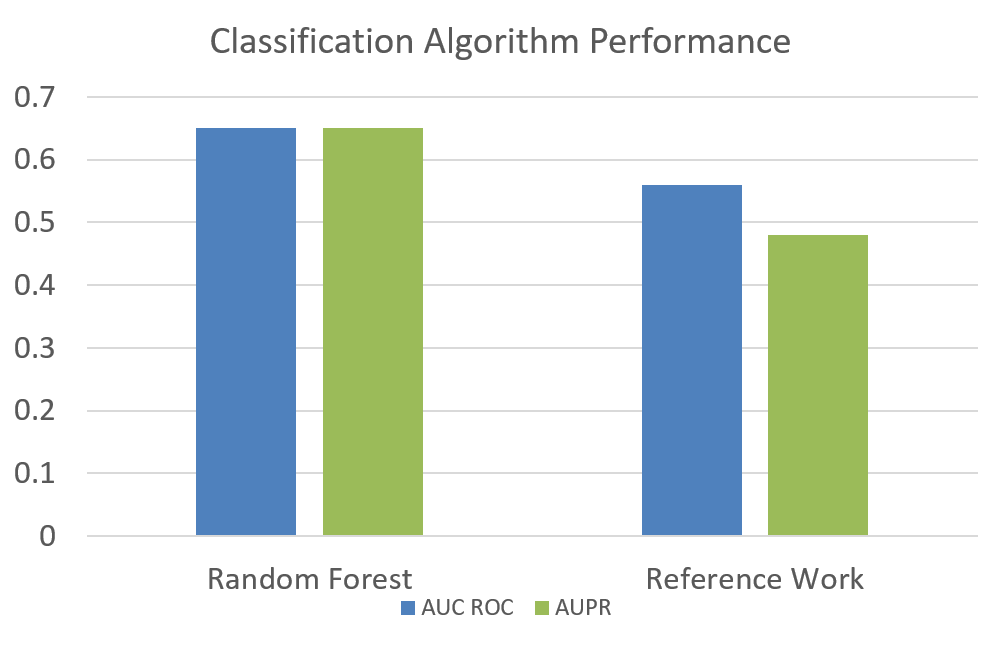
\includegraphics[width=\textwidth]{./Figures/first_res.png}
  \caption{Results from a simple Random Forest Classifier}
  \label{fig:first_res}
\end{figure}
Using Random Forest with EAM, improved our results to an AUC of 0.76 in comparison of 0.56 obtained by P.Schwab \cite{schwab2018phonemd} on Voice Data as shown in Figure \ref{fig:second_res}
\begin{figure}[htbp]
  \centering
  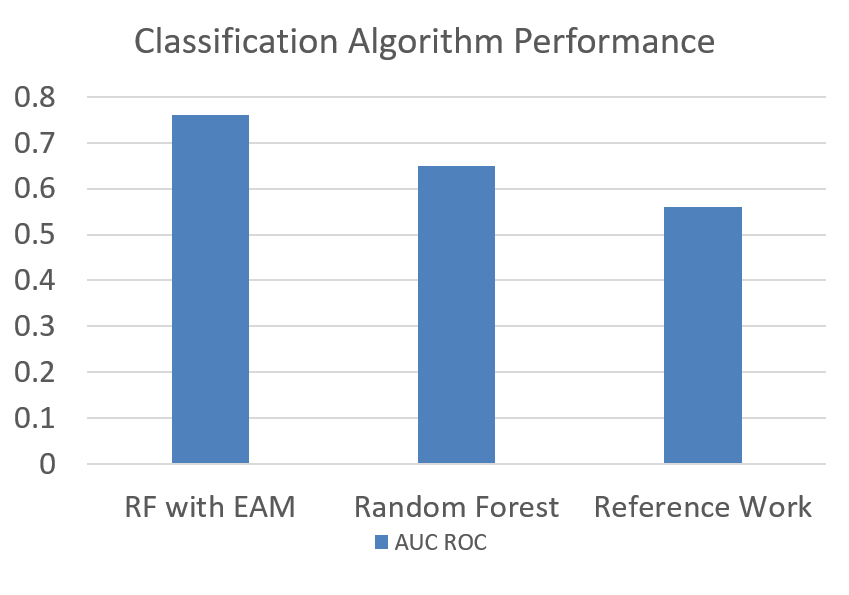
\includegraphics[width=\textwidth]{./Figures/second_res.png}
  \caption{Results from a simple Random Forest Classifier Alongwith EAM}
  \label{fig:second_res}
\end{figure}
\subsubsection{Results using Spline CNN}
The next logical step was to replace recording-level with a CNN to skip the pre-processing and feature Extraction step. This improved our measure to an AUC ROC of 0.89 with EAM for 3 recordings per patient as shown in Figure \ref{fig:third_res}
\begin{figure}[htbp]
  \centering
  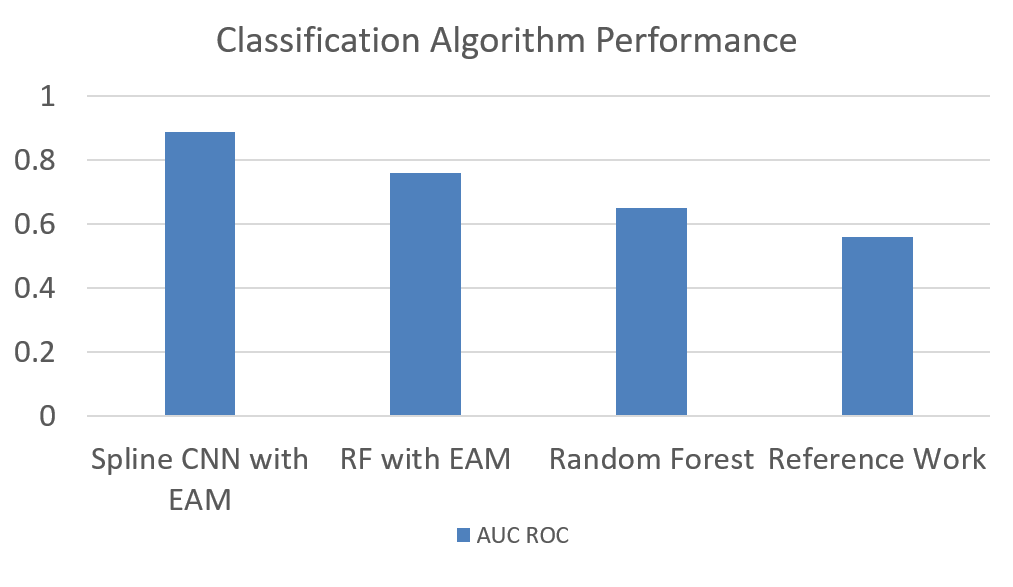
\includegraphics[width=\textwidth]{./Figures/third_res.png}
  \caption{Results from a Spline CNN Alongwith EAM}
  \label{fig:third_res}
\end{figure}
\subsubsection{Results Using Different Values of Recordings per Person}
The number of recordings per person were also changed and the results were recorded. As we can see that this change does not affect the performance very significantly,yet maximum performance was obtained at 3 recordings per person as shown in Figure \ref{fig:fourth_rse}.
\begin{figure}[htbp]
  \centering
  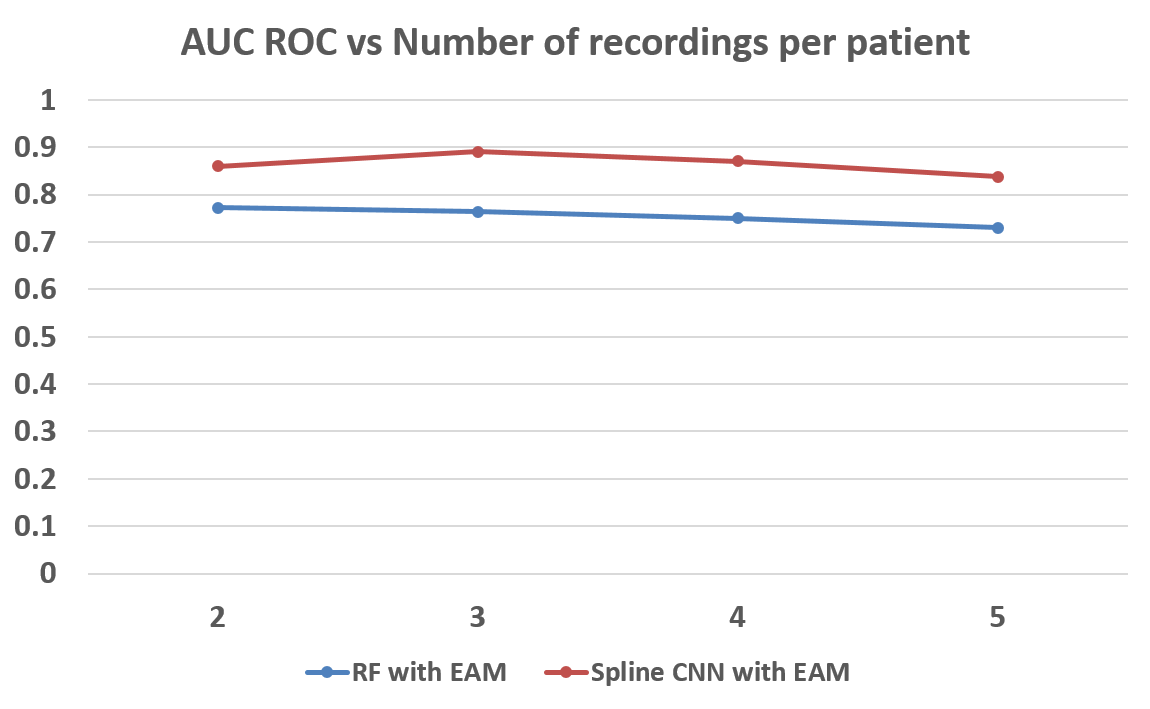
\includegraphics[width=\textwidth]{./Figures/fourth_rse.png}
  \caption{Change in Performace with Respect to Number of Recordings per Person}
  \label{fig:fourth_rse}
\end{figure}
The data composition was also changed when we changed the number of recordings per person which is illustrated in Figure \ref{fig:fifth_res}
\begin{figure}[htbp]
  \centering
  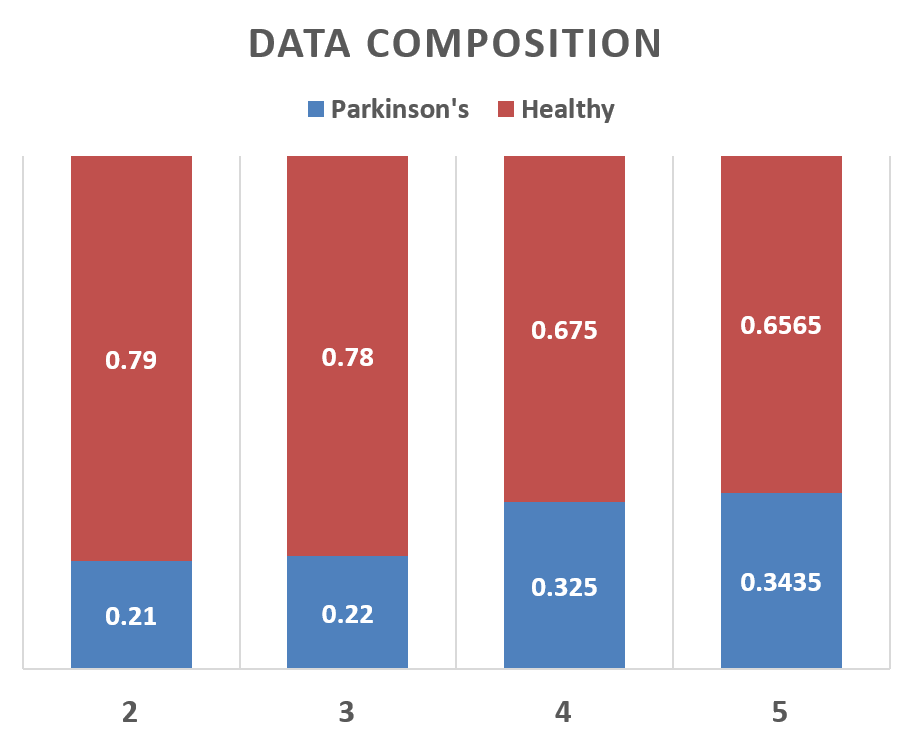
\includegraphics[width=\textwidth]{./Figures/fifth_res.png}
  \caption{Data Composition as we change the number of recordings per patient}
  \label{fig:fifth_res}
\end{figure}
\section{Result Analysis And Outlook}
\subsection{Application in Communication Systems}
The major stumbling block identified by our results is the need for training data. Our generalization error is made up of 2 components: Bias Error and Variance Error. While bias error can be decreased by making the model more complex, variance error cannot be decreased without increasing the amount of training data. For single user detection, when the channel was unvarying across frames, our neural network did not need to learn the channel distribution, and therefore a small number of training messages sufficed. However, as we increased the number of channel instances, the DNN needed to learn the underlying distribution of the channel and consequently required a large amount of training data. That is why for an unchanging, channel, our DNN performed the best, while for a changing channel it performed the worst. Table \ref{tbl:train_single_user} shows that as we increase the amount of training data, the performance of the neural network starts to improve.\\
\begin{table}[htbp]
  \centering
  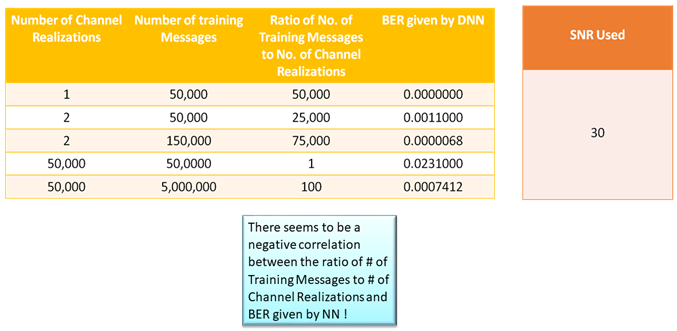
\includegraphics[width=\textwidth]{./Figures/train_single_user.png}
  \caption{Effect of increasing the Training Data for Single User Detection}
  \label{tbl:train_single_user}
\end{table}
Similarly, Table \ref{tbl:train_multi_user} convincingly suggests at lower amounts training data, the performance of the neural network is at par with the theoretical method that estimates the channel with Least Squares. However if we increase the number of training messages, the performance of the DNN improves, and it tries to approach the theoretical limit calculated by using the exact channel response which had been saved and loaded from a .csv file.  
\begin{table}[htbp]
  \centering
  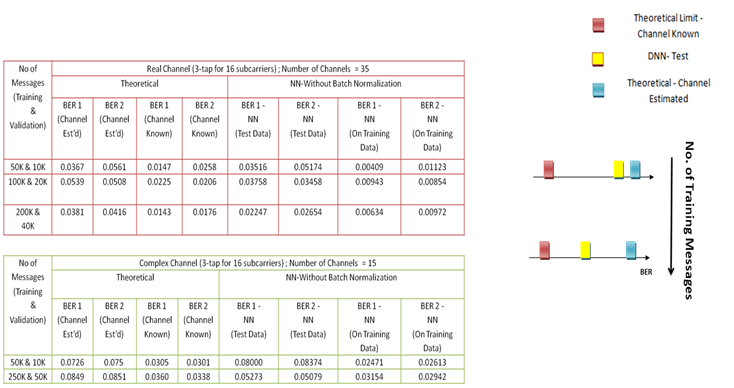
\includegraphics[width=\textwidth]{./Figures/train_multi_user.png}
  \caption{Effect of increasing the Training Data for Multi-User Detection}
  \label{tbl:train_multi_user}
\end{table}
\subsection{Application in Bioinformatics}
The major takeaway from our results is the importance of End-to-End Deep Learning as we have been able to improve quite a lot on the previous results by using the Spline-CNN. The main advantage of Spline-CNN is that it does not  need us to compute convolutional filters, but instead learns those filters based on data itself; we just initialize the filters as band-limited filters with the help of splines, and the rest is learned by the Network itself.\\
However, for End-to-End Deep Learning, here, we also face the same problem of the requirement of large amounts of data. This trend can be observed in Figure \ref{fig:fourth_rse} because as we increase the number of recordings per person, the results show a trend of decreasing performance. This is due to the decreasing amount of data we have available when we increase the number of recordings per person as there are fewer people who have recorded that many number of recordings or more. We can observe this trend in the number of recordings histogram in Figure \ref{fig:park_asymm}. % Experiment 1

% Chapter 3

\chapter{Cost Analysis, Conclusion, and Future Recommendations} % Write in your own chapter title
\label{Chapter5}
\lhead{} % Write in your own chapter title to set the page header

\section{Application in Communication Systems}
One of the major drawbacks of using the Neural Networks is that when the applications require a large amount of training data, the power and the specifications of the hardware required to go up exponentially. The more complexity we add to our model of the communication system, the more complicated becomes the architecture required. For example, in multi-user detection, when we moved from 16 subcarrier system to a more standard 64 sub-carrier systems, we had to increase the number of neurons by a factor of 4, and we had to increase the amount of training data by a factor of 10. The training required High-Performance Computing, and despite that, it took at least a week.  One positive outcome of this is that out of 2128 ($\approx 1038$) possible training messages which could be fed to our 64 subcarrier system, we at most require a very small subset of about tens of million distinct messages. This means that our network indeed learns the inverse of the transformation which mapped the bits to the received signal. Also, in terms of cost, big companies that are working in the field of communication do have powerful hardware at their disposal, which means that they will be able to train the network without the cost of any new hardware installation or purchase. One area of concern may be the power consumption of the hardware while training the network. But we must remember that we have to train the network only once to obtain the optimal weights of the model, which we can copy to and store in millions of devices. In other words, once we have trained the network, we can use a microcontroller or a chipset of negligible cost and power to do inference.


Nonetheless, it would be pertinent to mention that the system model our network uses is very rudimentary and simple. The neural network is trained at a constant SNR; the noise is AWGN, and the channel is drawn from a single Gaussian distribution; the bits are generated randomly too, and so the resultant symbols in the frame don’t have any covariance between them (On second thought, things could have been less complicated as covariance between symbols would have allowed us to use LSTM network who have a superior performance for sequence-2-sequence transformation.) To train our neural network for practical use, we could use more realistic channel models such as WINNER II. Also, we could change the SNR gradually but continuously to mimic real-time use of communication systems. Moreover, instead of generating the bits randomly, we could use data bits obtained from video, audio, or other documents to make the network more accurate. 

One area that has the potential for investigation is to decrease in pilot length. For Single-User Detection, when the pilot length is small, the performance of the neural network degrades less than that of traditional methods \cite{ye2018power}. Unfortunately, we failed to observe this trend for multi-user detection. Our future work aims to find improvements in the architecture, and find the optimal amount of training data so that we obtain this trend in the multi-user detection as well. 

\section{Application in Bioinformatics}
Our systems may have performed exceptionally well in terms of Area Under Receiver Operating Curve (AUC) as illustrated in Figure \ref{fig:third_res}, however, if we look at the sensitivity and specificity measures of the data as defined below:
$$Sensitivity = \frac{TP}{TP + FN}$$
$$Specificity = \frac{TN}{TN + FP}$$
In our context:
\begin{itemize}
\item $TP$ = True Positives = Number of Parkinson's Patients predicted as Parkinson's Patients
\item $TN$ = True Negatives = Number of Healthy People predicted as Healthy People
\item $FP$ = False Positives = Number of Parkinson's Patients predicted as Healthy People
\item $FN$ = False Negatives = Number of Healthy People predicted as Parkinson's Patients
\end{itemize}
Using this measure, we obtain the results illustrated in Figure \ref{fig:sens}. We see that they are not performing very well as the maximum sensitivity we were able to obtain is 0.41 which is not a very good result for providing a very good measure for providing Parkinson's predictions.
\begin{figure}[htbp]
  \centering
  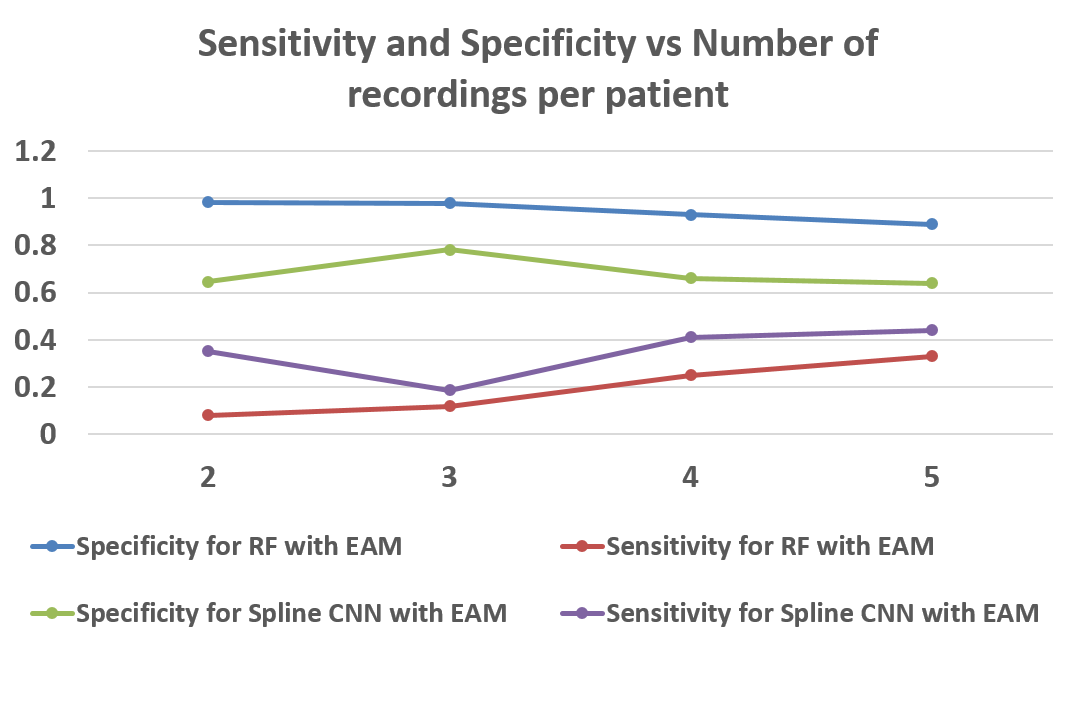
\includegraphics[width=\textwidth]{./Figures/park_sens_spec.png}
  \caption{Change in Sensitivity and Specificity as we change the number of recordings per person}
  \label{fig:sens}
\end{figure}
We believe that this is due to the following reasons:
\begin{itemize}
\item The data is highly imbalanced and stays so even when we change the recordings per patient as illustrated in Figure \ref{fig:fifth_res}. 
\item When we increase the number of recordings per patient, it seems to become less imbalanced, but at the same time, we have a lesser amount of data available, as there are fewer people who have recorded that many number of recordings or more. We can observe this trend in the number of recordings histogram in Figure \ref{fig:park_asymm}.
\end{itemize}
We aim to fight this trend either by optimizing our models for more sensitivity or by adding other modes (types) of activities data in the architecture as well. This way, the other activities data can help augment our predictions and improve them giving us a more robust model in terms of sensitivity and specificity as well. % Experiment 2

%\input{./Chapters/Chapter6} % Results and Discussion

%\input{./Chapters/Chapter7} % Conclusion

%% ----------------------------------------------------------------
\label{References}
\lhead{}  % Change the left side page header to "References"
\renewcommand\bibname{References}
\bibliographystyle{IEEEtran}  % Use "unsrtnat" BibTeX style for formatting the references

\bibliography{references}  % The references information are stored in the file named "references.bib"
\begin{comment}
%% ----------------------------------------------------------------
\setstretch{1.3}  % It is better to have smaller font and larger line spacing than the other way round

% Define the page headers using the FancyHdr package and set up for one-sided printing
\fancyhead{}  % Clears all page headers and footers
\rhead{\thepage}  % Sets the right side header to show the page number
\lhead{}  % Clears the left side page header

\pagestyle{fancy}  % Finally, use the "fancy" page style to implement the FancyHdr headers


%% Select only one of the certification pages  
%\CertificationMSc{}
\CertificationBSc{}
\clearpage  % Certification ended, now start a new page


%% ----------------------------------------------------------------
% End of the pre-able, contents and lists of things
% Begin the Dedication page
\setstretch{1.3}  % Return the line spacing back to 1.3
\pagestyle{empty}  % Page style needs to be empty for this page
\dedicatory{For/Dedicated to/To my\ldots}


%% ----------------------------------------------------------------
\pagestyle{fancy}  %The page style headers have been "empty" all this time, now use the "fancy" headers as defined before to bring them back

%% ----------------------------------------------------------------
\setstretch{1.5}  % Set the line spacing to 1.5, this makes the following tables easier to read
\clearpage  % Start a new page
\lhead{\emph{Abbreviations}}  % Set the left side page header to "Abbreviations"
\listofsymbols{ll}  % Include a list of Abbreviations (a table of two columns)
{
% \textbf{Acronym} & \textbf{W}hat (it) \textbf{S}tands \textbf{F}or \\
\textbf{LAH} & \textbf{L}ist \textbf{A}bbreviations \textbf{H}ere \\
}

%% ----------------------------------------------------------------
% Now begin the Appendices, including them as separate files

\addtocontents{toc}{\vspace{2em}} % Add a gap in the Contents, for aesthetics

\appendix % Cue to tell LaTeX that the following 'chapters' are Appendices

% Appendix A

\chapter{Introduction to Latex}
\label{AppendixA}
\lhead{Appendix A. \emph{Introduction to Latex}}

The material provided in this appendix is taken from \\
\href{http://www.sunilpatel.co.uk/thesistemplate.php}{\texttt{http://www.sunilpatel.co.uk/thesistemplate.php}}

\section{Learning \LaTeX{}}

\LaTeX{} is not a WYSIWYG (What You See is What You Get) program, unlike word processors such as Microsoft Word or Corel WordPerfect. Instead, a document written for \LaTeX{} is actually a simple, plain text file that contains \emph{no formatting}. You tell \LaTeX{} how you want the formatting in the finished document by writing in simple commands amongst the text, for example, if I want to use \emph{italic text for emphasis}, I write the `$\backslash$\texttt{emph}\{\}' command and put the text I want in italics in between the curly braces. This means that \LaTeX{} is a ``mark-up'' language, very much like HTML.

\subsection{A (not so short) Introduction to \LaTeX{}}

If you are new to \LaTeX{}, there is a very good eBook -- freely available online as a PDF file -- called, ``The Not So Short Introduction to \LaTeX{}''. The book's title is typically shortened to just ``lshort''. You can download the latest version (as it is occasionally updated) from here:\\
\href{http://www.ctan.org/tex-archive/info/lshort/english/lshort.pdf}{\texttt{http://www.ctan.org/tex-archive/info/lshort/english/lshort.pdf}}

It is also available in several other languages. Find yours from the list on this page:\\
\href{http://www.ctan.org/tex-archive/info/lshort/}{\texttt{http://www.ctan.org/tex-archive/info/lshort/}}

It is recommended to take a little time out to learn how to use \LaTeX{} by creating several, small `test' documents. Making the effort now means you're not stuck learning the system when what you \emph{really} need to be doing is writing your thesis.

\subsection{A Short Math Guide for \LaTeX{}}

If you are writing a technical or mathematical thesis, then you may want to read the document by the AMS (American Mathematical Society) called, ``A Short Math Guide for \LaTeX{}''. It can be found online here:\\
\href{http://www.ams.org/tex/amslatex.html}{\texttt{http://www.ams.org/tex/amslatex.html}}\\
under the ``Additional Documentation'' section towards the bottom of the page.

\subsection{Common \LaTeX{} Math Symbols}
There are a multitude of mathematical symbols available for \LaTeX{} and it would take a great effort to learn the commands for them all. The most common ones you are likely to use are shown on this page:\\
\href{http://www.sunilpatel.co.uk/latexsymbols.html}{\texttt{http://www.sunilpatel.co.uk/latexsymbols.html}}

You can use this page as a reference or crib sheet, the symbols are rendered as large, high quality images so you can quickly find the \LaTeX{} command for the symbol you need.



\subsection{Figures}

There will hopefully be many figures in your thesis (that should be placed in the `Figures' folder). The way to insert figures into your thesis is to use a code template like this:
\begin{verbatim}
\begin{figure}[htbp]
  \centering
    
\includegraphics[width = 1.5in]{./Figures/lums_logo.png}
    \rule{35em}{0.5pt}
  \caption{The UET Laore logo.}
  \label{fig:uet_logo}
\end{figure}
\end{verbatim}
Also look in the source file. Putting this code into the source file produces the picture of the UET logo that you can see in the figure below.

\begin{figure}[htbp]
	\centering
		
\includegraphics[width = 1.5in]{./Figures/lums_logo.png}
		\rule{35em}{0.5pt}
	\caption{The UET Laore logo.}
	\label{fig:uet_logo}
\end{figure}

Sometimes figures don't always appear where you write them in the source. The placement depends on how much space there is on the page for the figure. Sometimes there is not enough room to fit a figure directly where it should go (in relation to the text) and so \LaTeX{} puts it at the top of the next page. Positioning figures is the job of \LaTeX{} and so you should only worry about making them look good!

Figures usually should have labels just in case you need to refer to them (such as in figure \ref{fig:uet_logo}). The `$\backslash$\texttt{caption}' command contains two parts, the first part, inside the square brackets is the title that will appear in the `List of Figures', and so should be short. The second part in the curly brackets should contain the longer and more descriptive caption text.

The `$\backslash$\texttt{rule}' command is optional and simply puts an aesthetic horizontal line below the image. If you do this for one image, do it for all of them.

The \LaTeX{} Thesis Template is able to use figures that are either in the PDF or JPEG file format. It is recommended that you read this short guide on how to get the best out of figures in \LaTeX{}, available here:\\
\href{http://www.sunilpatel.co.uk/texhelp5.html}{\texttt{http://www.sunilpatel.co.uk/texhelp5.html}}

Though it is geared more towards users of Mac and OS X systems, much of the advice applies to creating and using figures in general. It also explains why the PDF file format is preferred in figures over JPEG.

\subsection{Typesetting mathematics}

If your thesis is going to contain heavy mathematical content, be sure that \LaTeX{} will make it look beautiful, even though it won't be able to solve the equations for you.

The ``Not So Short Introduction to \LaTeX{}'' (available \href{http://www.ctan.org/tex-archive/info/lshort/english/lshort.pdf}{here}) should tell you everything you need to know for most cases of typesetting mathematics. If you need more information, a much more thorough mathematical guide is available from the AMS called, ``A Short Math Guide to \LaTeX{}'' and can be downloaded from:\\
\href{ftp://ftp.ams.org/pub/tex/doc/amsmath/short-math-guide.pdf}{\texttt{ftp://ftp.ams.org/pub/tex/doc/amsmath/short-math-guide.pdf}}

There are many different \LaTeX{} symbols to remember, luckily you can find the most common symbols \href{http://www.sunilpatel.co.uk/latexsymbols.html}{here}. You can use the web page as a quick reference or crib sheet and because the symbols are grouped and rendered as high quality images (each with a downloadable PDF), finding the symbol you need is quick and easy.

You can write an equation, which is automatically given an equation number by \LaTeX{} like this:
\begin{verbatim}
\begin{equation}
E = mc^{2}
  \label{eqn:Einstein}
\end{equation}
\end{verbatim}

This will produce Einstein's famous energy-matter equivalence equation:
\begin{equation}
E = mc^{2}
\label{eqn:Einstein}
\end{equation}

All equations you write (which are not in the middle of paragraph text) are automatically given equation numbers by \LaTeX{}. If you don't want a particular equation numbered, just put the command, `$\backslash$\texttt{nonumber}' immediately after the equation.


\section{Sectioning and Subsectioning}

You should break your thesis up into nice, bite-sized sections and subsections. \LaTeX{} automatically builds a table of Contents by looking at all the `$\backslash$\texttt{chapter}$\{\}$', `$\backslash$\texttt{section}$\{\}$' and `$\backslash$\texttt{subsection}$\{\}$' commands you write in the source.

The table of Contents should only list the sections to three (3) levels. A `$\backslash$\texttt{chapter}$\{\}$' is level one (1). A `$\backslash$\texttt{section}$\{\}$' is level two (2) and so a `$\backslash$\texttt{subsection}$\{\}$' is level three (3). In your thesis it is likely that you will even use a `$\backslash$\texttt{subsubsection}$\{\}$', which is level four (4). Adding all these will create an unnecessarily cluttered table of Contents and so you should use the `$\backslash$\texttt{subsubsection$^{*}\{\}$}' command instead (note the asterisk). The asterisk ($^{*}$) tells \LaTeX{} to omit listing the subsubsection in the Contents, keeping it clean and tidy.
	% Appendix Title

%\input{./Chapters/AppendixB} % Appendix Title

%\input{./Chapters/AppendixC} % Appendix Title

\addtocontents{toc}{\vspace{2em}}  % Add a gap in the Contents, for aesthetics
\backmatter

\end{comment}
\end{document}  % The End
%% ----------------------------------------------------------------
